%%%%%%%%%%%%%%%%%%%%%%%%%%%%%%%%%%%%%%%%%%%%%%%%%%%%%%%%%%
%
% Vzor pro sazbu kvalifikační práce
%
% Západočeská univerzita v Plzni
% Fakulta aplikovaných věd
% Katedra informatiky a výpočetní techniky
%
% Petr Lobaz, lobaz@kiv.zcu.cz, 2016/03/14
%
%%%%%%%%%%%%%%%%%%%%%%%%%%%%%%%%%%%%%%%%%%%%%%%%%%%%%%%%%%

% Možné jazyky práce: czech, english
% Možné typy práce: BP (bakalářská), DP (diplomová)
\documentclass[czech,DP]{thesiskiv}

% Definujte údaje pro vstupní strany
%
% Jméno a příjmení; kvůli textu prohlášení určete, 
% zda jde o mužské, nebo ženské jméno.
\author{Zdeněk Valeš}
\declarationmale

%alternativa: 
%\declarationfemale

% Název práce
\title{Určování nahraditelnosti a\\kompatibility webových služeb}

% 
% Texty abstraktů (anglicky, česky)
%
\abstracttexten{The text of the abstract (in English). It contains the English translation of the thesis title and a short description of the thesis.}

\abstracttextcz{Text abstraktu (česky). Obsahuje krátkou anotaci (cca 10 řádek) v češtině. Budete ji potřebovat i při vyplňování údajů o bakalářské práci ve STAGu. Český i anglický abstrakt by měly být na stejné stránce a měly by si obsahem co možná nejvíce odpovídat (samozřejmě není možný doslovný překlad!).
}

% Na titulní stranu a do textu prohlášení se automaticky vkládá 
% aktuální rok, resp. datum. Můžete je změnit:
%\titlepageyear{2016}
%\declarationdate{1. března 2016}

% Ve zvláštních případech je možné ovlivnit i ostatní texty:
%
%\university{Západočeská univerzita v Plzni}
%\faculty{Fakulta aplikovaných věd}
%\department{Katedra informatiky a výpočetní techniky}
%\subject{Bakalářská práce}
%\titlepagetown{Plzeň}
%\declarationtown{Plzni}

%%%%%%%%%%%%%%%%%%%%%%%%%%%%%%%%%%%%%%%%%%%%%%%%%%%%%%%%%%
%
% DODATEČNÉ BALÍČKY PRO SAZBU
% Jejich užívání či neužívání záleží na libovůli autora 
% práce
%
%%%%%%%%%%%%%%%%%%%%%%%%%%%%%%%%%%%%%%%%%%%%%%%%%%%%%%%%%%

% Zařadit literaturu do obsahu
\usepackage[nottoc,notlot,notlof]{tocbibind}

% Umožňuje vkládání obrázků
\usepackage[pdftex]{graphicx}
\graphicspath{{./img/}}

% Odkazy v PDF jsou aktivní; navíc se automaticky vkládá
% balíček 'url', který umožňuje např. dělení slov
% uvnitř URL
\usepackage[pdftex]{hyperref}
\hypersetup{colorlinks=true,
  unicode=true,
  linkcolor=black,
  citecolor=black,
  urlcolor=black,
  bookmarksopen=true}

% Při používání citačního stylu csplainnatkiv
% (odvozen z csplainnat, http://repo.or.cz/w/csplainnat.git)
% lze snadno modifikovat vzhled citací v textu
\usepackage[numbers,sort&compress]{natbib}


% na seznam zktratek
\usepackage{longtable}
\newcommand\nomenclature[2]{#1 & #2 \\}

% víceřádkové buňky v tabulce
\usepackage{makecell}

\renewcommand\theadalign{bc}
\renewcommand\theadfont{\bfseries}
\renewcommand\theadgape{\Gape[4pt]}
\renewcommand\cellgape{\Gape[4pt]}

% delta-eq
\usepackage{amssymb}

% zdroják
\usepackage{listings}

%%%%%%%%%%%%%%%%%%%%%%%%%%%%%%%%%%%%%%%%%%%%%%%%%%%%%%%%%%
%
% VLASTNÍ TEXT PRÁCE
%
%%%%%%%%%%%%%%%%%%%%%%%%%%%%%%%%%%%%%%%%%%%%%%%%%%%%%%%%%%
\begin{document}
%
\maketitle
\tableofcontents

\chapter{Úvod}

% k čemu je práce dobrá
% co text práce obahuje
% use casy

 - Webové služby jsou v dnešní době stále populárnější součást vývoje aplikací
 - Spousta firem chce zpřístupnit svá data, proto poskytuje veřejné i neveřejné rozhraní pro přístup k nim
 - Webové služby také tvoří velkou část podnikových procesů
 - Existuje také spousta různých typů služeb, z nichž některé jsou popsané strojově čitelnými jazyky, jiné vůbec žádnými
 - Architektura Microservice je založe na systému volně propojených webových služeb
 - Komunikace mezi službami závisí na rozhraní, v případě, že dojde k změně v implementaci služby, jež přímo naruší kontrakt daný rozhraním, může na straně konzumenta služby vzniknout problém s kompatibilitou, který se může projevit například výpadkem služby
 - Aplikace konzumující službu také může potřebovat přepnout poskytovatele stávající služby ať už kvůli přechodu mezi regiony, nebo dočasnému výpadku
 - Aby nedošlo k chybám při tomto přepnutí, je nutné kontrolovat vzájemnou kompatibilitu těchto služeb
 - Systém CRCE vyvíjený na ZČU je schopný indexace komponent a ukládání jejich metadat
 - V rámci prací Bc. Hessové a Bc. Pejřimovského vznikla rozšíření CRCE schopná transformovat rozhraní různých typů služeb do jednotného datového modelu
 - Cílem mé práce je na tyto práce navázat využitím metadat a  na základě rozdílů získaných jejich porovnáním rozhodnout o vzájemné kompatibilitě webových služeb, které reprezentují
 - V textu práce jsou postupně představeny webové služby a technologie ki jejich realizaci
 - Následně je představen koncept datových typů a jejich vzájemného porovnání
 - Druhá část práce se zabývá návrhem a implementací porovnávacího algoritmu jako rozšiřujícího modulu pro systém CRCE
 - Na závěr je ověřena funkčnost modulu a jeho integrace do CRCE na testovacích datech 

\chapter{Webové služby}
\label{sec:web-services-principles}

V této kapitole jsou definovány webové služby a související pojmy. Dále je popsán protokol HTTP, na kterém je primárně postavena komunikace mezi službami a stručně jsou také uvedeny formáty pro přenos dat. V druhé části kapitoly jsou představeny dva hlavní přístupy k realizaci služeb a na závěr je uveden výčet formátů použitých ke strojově čitelnému popisu rozhraní služeb.

%co je v téhle kapitole:
%
% - co jsou to webové služby
% - k čemu webové služby jsou
% - co je to REST (protože se to přímo dotýká mé práce)
% - co je to API
% - protokoly skrze které se s WS komunikuje
% - strojově čitelné formáty popisu ws

\section{Webová služba}
% \cite{w3cWsDesignIssues}
% v citovaném článku je spousta zajímavých informací o WS, např "The fact that data is exchanged for business purposes and between different social entities means that accountability is required, rather than just reliable transmission. "



% pojem webová služba má různé významy \cite{w3cWsDesignIssues}
% je třeba je n v rámci této práce jasně definovat
% W3C používá jendu difnici \cite{w3cWsDesignIssues}

Pojem 'webová služba' může mít odlišné významy\cite{w3cWsDesignIssues} a existuje pro něj také spousta definic, z nichž některé jsou více či méně vhodné pro tento text. Například konsorcium W3C\footnote{World Wide Web Consorcium} definuje pojem webová služba následovně\cite{w3cWsArch}:


 % A Web service is a software system designed to support interoperable machine-to-machine interaction over a network. It has an interface described in a machine-processable format (specifically WSDL). Other systems interact with the Web service in a manner prescribed by its description using SOAP messages, typically conveyed using HTTP with an XML serialization in conjunction with other Web-related standards.
\begin{quote}
	Webová služba je softwarový systém navržený pro podporu mezistrojové komunikace po síti. Webová služba má rozhraní, které je popsáno ve strojově čitelném formátu (konkrétně WSDL). Ostatní systémy interagují s webovými službami předepsaným způsobem za použití zpráv protokolu SOAP, které jsou typicky zprostředkované protokolem HTTP s využitím serializace XML a dalších webových standardů.
\end{quote}

% ta není dobrá protože ... 

Tato definice je pro účely mé práce problematická z několika důvodů. Prvním z nich je omezení formátu popisu služby pouze na WSDL. Strojově čitelný popis rozhraní sice snižuje náročnost vytvoření klienta pro danou službu, nicméně WSDL není jediným takovým formátem a netřeba tedy z definice vyloučit služby používající jiné formáty jako například WADL nebo JSON-WSP, jež přímo souvisí s mou prací. Závislost na jednom konkrétním formátu také nemusí být výhodná z hlediska budoucího vývoje, protože nezohledňuje možnost příchodu jiného formátu nebo změny přístupu k webovým službám obecně. WSDL do verze 1.1 například neumožňovalo popis REST služeb, ty byly zohledněny až ve verzi 2.0\cite{restWsdl}.  

Definice dále svazuje implementaci webové služby s použitím konkrétního protokolu pro výměnu dat, v tomto případě SOAP, čímž opět nezahrnuje služby používající jakékoliv jiné protokoly. I zde platí nevýhoda takové vazby v kontextu budoucího vývoje, jež byla zmíněna v předchozím odstavci. Webová služba by například přestala být webovou službou, pokud by došlo k změně protokolu pro výměnu dat ze SOAP na JSON-RPC, což není žádoucí.

Posledním důvodem je vymáhání použití XML jako jediného formátu pro přenos dat i přes rostoucí popularitu jiných formátů, jako například JSON nebo v poslední době YAML. Není také výjimkou, že webové služby podporují více formátů pro serializaci dat a specifikace jednoho konkrétního formátu v definici tedy není nutná. 

% a proto je webová služba zadefinována takto
Z uvedených důvodů je potřeba zavést vhodnější definici s volnějšími kritérii tak, aby webové služby co možná nejméně omezovala. Definici, která služby popisuje primárně skrze užití komunikačního protokolu HTTP ve své knize nabízí R. Daigneau \cite{fromObjectsToWs}: 

%	Web services provide the means to integrate disparate systems and expose reusable business functions over HTTP. They either leverage HTTP as a simple transport over which data is carried (e.g., SOAP/WSDL services) or use it as a complete application protocol that defines the semantics for service behavior (e.g., RESTful services).
\begin{quote}
	Webové služby poskytují prostředky pro integraci různorodých systémů a zpřístupňují znovupoužitelné business funkce skrze HTTP. HTTP je použito buď jako jednoduchý komunikační protokol, skrze který jsou přenášena data (např. SOAP/WSDL služby), nebo jako kompletní aplikační protokol, jež definuje sémantiku chování služby (např. RESTful služby).
\end{quote}

Tato definice netrpí výše zmíněnými nedostatky a zahrnuje webové služby jimiž se tato práce zabývá. Proto jsem se rozhodl ji využít pro účely mé práce a nebude-li určeno jinak, pojem 'webová služba' v tomto textu odpovídá zmíněné definici. S webovými službami se váže několik dalších pojmů, které jsou v průběhu textu užívány, a pro úplnost jsou zde taktéž definovány:

% definovat další pojmy jako
% - pokytovatel služby
% - konzument služby
% - endpoint ve službě
% - operace ve službě
% - service ve službě
%	- důvod použití pojmu service: při překladu do češtiny by mohl pojem kolidovat s pojmem 'webová služba', proto je pro element WSDL označující část SOAP služby použit pojem service

\begin{itemize}
	\item \textbf{Poskytovatel služby}: server na kterém je služba dostupná, případě organizace, která ji spravuje,
	\item \textbf{Konzument služby}: klient využívající službu, typicky se jedná o aplikaci,
	\item \textbf{Endpoint}: Jedna konkrétní operace služby, případě URI na které je dostupný nějaký zdroj nebo celá služba,
	\item \textbf{Operace}: Operace webové služby, v tomto textu používáno ve stejném významu jako endpoint,
	\item \textbf{Service}: element \verb|service| v popisu WSDL, při překladu do češtiny (služba) by mohl pojem kolidovat s pojmem 'webová služba', proto je pro element WSDL označující část služby ponechán anglický tvar service,
	\item \textbf{API}: Rozhraní webové služby.
\end{itemize}

Ve své práci jsem se zabýval dvěma velkými skupinami webových služeb rozdělených podle přístupu k jejich architektuře. Těmi jsou RPC\footnote{Remote Procedure Call}-orientované služby a RESTové služby. Oba přístupy včetně technologií použitých k jejich realizaci jsou rozvedené v následujících sekcích.

\subsection{Použití webových služeb}

Samotný pojem služba z technického pohledu typicky označuje funkcionalitu, jež vykonává nějakou podnikovou operaci, zajišťuje přístup k souborům, nebo obstarává generickou funkcionalitu jako například přihlášení do systému. Webové služby umožňují tyto zpřístupnit různorodým klientům jako jsou například webový prohlížeč nebo mobilní aplikace, nezávisle na technologiích použitých k jejich realizaci.

% \cite{fromObjectsToWs}
% ws jsou jednoduché na použití, ke komunikaci stačí pouze HTTP, JSON/XML pro výměnu dat a znalost protokolu
% to nutně neplatilo u předchůdců, například Shared Objects
% díky tomu jsou služby snadno propojitelné a lze je skládat do větších celků za účelem realizace komplexních operací (funkcionalit)
Ve srovnání s alternativami jako například distribuované objekty jsou webové služby snazší na použití, zejména kvůli jednoduché komunikaci skrze protokol HTTP a standardizované serializaci dat do formátů jako XML nebo JSON. Použitím jednotného komunikačního kanálu (HTTP) je také docíleno oddělení implementace klienta od služby a tím i větší nezávislosti mezi nimi. Díky tomu jsou webové služby snadno propojitelné a lze je tak skládat do větších celků za účelem realizace komplexních procesů\cite{fromObjectsToWs}.

% služby vytváří/nastolují vrstvu abstrakce mezi samotnou implementací služby a klientem
% tím je docíleno volné vazby a jak služba tak klient se mohou nezávisle vyvíjet, dokud nedojde ke změnám narušujícím kompatibilitu (to by chtělo rozepsat víc)
% tady lze zmínit např architekturu microservice
% z toho by se mohlo dát navázat na problém změny implementace/resp. rozhraní a tím vzniklé nekompatibility mezi službou, kterou očekává klient a službou, kterou server poskytuje
Architektura \textit{Microservices} této skutečnosti využívá a na aplikace nahlíží jako na systém volně propojených služeb, z nichž každá je nezávislá na ostatních a soustředí se na svou přidělenou úlohu. Tou může být například správa uživatelů, nebo analýza dat. Služby v této architektuře se také vyznačují vzájemně nezávislým vývojem \cite{microservices}, což může vést na problémy se vzájemnou kompatibilitou, pokud je například do nové verze služby zanesena změna mutující její rozhraní. Právě tímto tématem se v kontextu webových služeb zabývá má práce.


% taky by nebylo špatný popsat kdy dává použití WS smysl
% tím se zabývá podkapitola Web Service Considerations and Alternatives

\section{Techniky webových služeb}
\label{sec:ws-tech}

Tato podkapitola krátce představuje nejzákladnější techniky a protokoly určené k realizaci webových služeb. Z hlediska komunikace se jedná o protokol HTML a formáty XML a JSON sloužící k výměně dat a popisu rozhraní služeb.

% zmínit:
% zmínit RPC, SOAP
%- popis použitých technologií: XML, SOAP, WSDL
% někde zmínit, že se zde zaměřuji hlavně na dva druhy služeb:  RPC a REST 

%vzory:
%- RPC API
%- Message API
%- Resource API

%0Faktory ke zvážení při návrhu API\cite{wsApiStyles}: Zapouzdření, Kontrakt služby, Autonomnost 

%\begin{figure}[h]
%	\centering
%	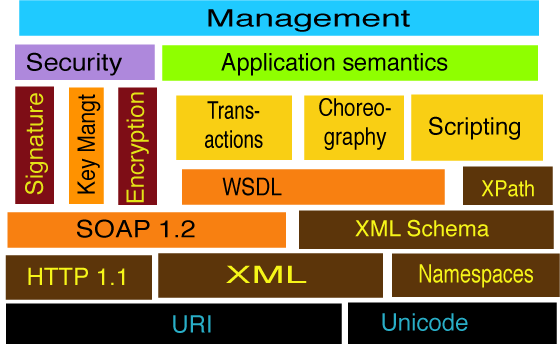
\includegraphics[width=\linewidth]{ws-tech-stack.png}
%	\caption{Technologie zahrnuté ve webových službách}
%	\label{fig:ws-tech-stack}	
%\end{figure}

\subsection{HTTP}

% úvod do sekce o HTTP
HTTP\footnote{Hypertext Transfer Protocol} je bezestavový protokol aplikační vrstvy určený pro distribuované hypermediální systémy a tvoří základ informačního systému WWW\footnote{World Wide Web}, který jej využívá od 90. let \cite{httpRfc}. Celkem bylo specifikováno pět verzí protokolu: 0.9, 1.0, 1.1, 2.0 a 3.0. Tato sekce se zabývá protokolem HTTP/1.1, neboť právě vlastnosti představené v této verzi jsou relevantní mé práci. Komunikace přes HTTP typicky probíhá skrze TCP/IP spojení na portu 80. 

% princip HTTP
Protokol je založen na principu volání-odpověď. Klient odešle žádost ve formě metody, identifikátoru a verze protokolu, následovanou tělem žádosti v MIME\footnote{Multipurpose Internet Mail Extensions} formátu. Identifikátor žádosti posílané klientem je tvořen URI\footnote{Uniform Resource Identifier}, což je sekvence znaků, která jasně určuje daný zdroj \cite{uriRfc}. Tělo může obsahovat informace o klientovi, modifikátory žádosti a data pro příjemce. Server odpoví statusem, jež zahrnuje verzi protokolu a kód výsledku žádosti (chyba, nebo úspěch). Ten je následovaný zprávou, rovněž ve formátu MIME, obsahující informace o serveru a případně tělo odpovědi s daty pro klienta \cite{httpRfc}.

% metody HTTP
HTTP definuje množinu metod, jejichž účelem je specifikovat konkrétní operaci, která by měla být provedená nad daným zdrojem, identifikovaným volaným URI. Výčet metod společně s popisem je uveden v tabulce \ref{tab:http-methods}.

\begin{table}[h]
	\centering
	\begin{tabular}{|l|c|c|}
		\hline
		Název & Popis užití & Idempotentní \\
		\hline
		\hline
		GET & Získání informace náležící volanému URI & ANO \\
		\hline
		HEAD & Identická GET, ale odpověď neobsahuje tělo & ANO \\
		\hline
		PUT & \makecell{Vytvoření nové, nebo aktualizace existující \\ entity odpovídající volanému URI }  & ANO \\
		\hline
		DELETE & Smazání zdroje identifikovaným volaným URI & ANO \\
		\hline
		OPTIONS & Získání informací o možnostech komunikace  & ANO \\
		\hline
		TRACE & Příjemce odešle zpět tělo přijaté zprávy & ANO \\
		\hline
		POST & \makecell{Vytvoření nových dat vztažených ke \\ zdroji identifikovaným volaným URI} & NE \\
		\hline
		CONNECT & Rezervovaný název & NE \\
		\hline		
	\end{tabular}
	\caption{Metody definované v HTTP protokolu}
	\label{tab:http-methods}
\end{table}

Implementace obsluhy metod sice záleží na konkrétním poskytovateli, nicméně HTTP definuje tzv. bezpečné metody, jež by měly označovat pouze operace určené k získání dat. Jedná se o metody GET a HEAD. Protokol u metod také zavádí vlastnost idempotentnosti pokud $N>0$ identických volání způsobí stejné vedlejší efekty jako pouhé jedno volání \cite{httpRfc}.


\subsection{Formáty pro přenos dat}

Služby komunikující protokolem HTTP si obvykle předávají data v textové podobě. Způsobů, jak taková data formátovat existuje mnoho, nicméně během mé práce jsem přišel do styku převážně s formáty XML a JSON, proto se zde zaměřím právě na ně. Zmíněné syntaxe nemusí být použity pouze k serializaci předávaných dat, ale také k popisu rozhraní samotné služby, jak bude ukázáno v části \ref{sec:api-description-formats}.

\subsubsection{XML}

Extensible markup language (dále jen XML) je značkovací jazyk určený k reprezentaci dokumentů ve formátu, který je čitelný pro stroj i člověka. První verze specifikace\footnote{https://www.w3.org/TR/REC-xml/} byla zveřejněna roku 1998 konsorciem W3C, které tento formát vyvíjí a spravuje. MIME typ pro označení XML je \verb|application/xml|.

Základními stavebními kameny jazyka XML jsou dokument, tagy, elementy a atributy. Dokument je definován jako datový objekt, jež se skládá z prologu označujícího verzi XML, jednoho kořenového elementu a případných dodatků. Všechny zmíněné části dokumentu musí odpovídat syntaxi jazyka XML. Element je logická jednotka dokumentu ohraničená tagy. Může být prázdný, nebo může vnořovat další elementy. Atributy jsou páry klíč-hodnota přiřazené elementu.

Příklad XML dokumentu je znázorněn na obrázku \ref{fig:xml-example}. Kořenovým elementem je v tomto případě \verb|quiz|, jež je ohraničený tagem \verb|<quiz>|. Jeho vnořeným elementem je \verb|qanda| obsahující atribut \verb|seq| s hodnotou \verb|1|.

\begin{figure}[h]
	\centering
	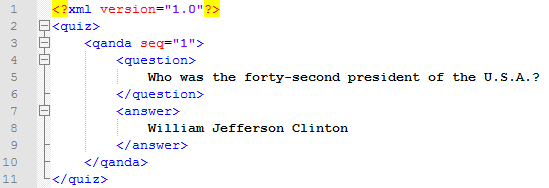
\includegraphics[width=12.5cm]{xml-example.png}
	\caption{Příklad XML dokumentu}
	\label{fig:xml-example}
\end{figure} 

\subsubsection{JSON} 
JavaScript object notation (dále jen JSON) je formát výměny dat vzešlý z části standardu jazyka JavaScript\footnote{https://www.ecma-international.org/publications/standards/Ecma-262-arch.htm} publikovaného v roce 1999. Samotný JSON byl poprvé standardizován specifikací ECMA-404\footnote{https://www.ecma-international.org/publications/standards/Ecma-404-arch.htm} v roce 2013. Stejně jako zmíněný XML, je i tento čitelný pro člověka a stroj.  MIME typ pro označení JSON je \verb|application/json|.

JSON je založen na dvou základních strukturách, jež by měly být podporovány většinou dnešních moderních programovacích jazyků. Těmito strukturami jsou kolekce párů klíč-hodnota zvaná \textit{objekt} a seřazený seznam hodnot zvaný \textit{pole}. Objekt je ohraničen složenými závorkami \verb|{|, \verb|}| a obsahuje neseřazený výčet párů klíč-hodnota. Klíč je od hodnoty oddělen dvojtečkou a celé páry jsou oddělené čárkami. Pole je ohraničeno hranatými závorkami \verb|[|, \verb|]| a obsahuje seřazený výčet hodnot, jež jsou vzájemně odděleny čárkou.

Obrázek \ref{fig:json-examle} obsahuje příklad JSON objektu analogickému ke XML dokumentu na obrázku \ref{fig:xml-example}. Kořenový objekt obsahuje klíč \verb|kviz|, ke kterému jako hodnota náleží pole otázek. Otázka je reprezentována objektem s hodnotami pro klíče \verb|seq|, \verb|question| a \verb|answer|.

\begin{figure}[h]
	\centering
	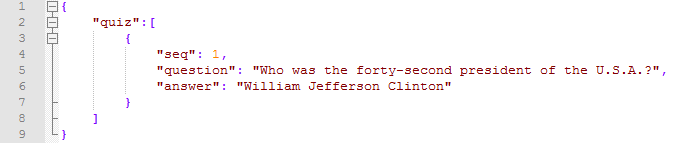
\includegraphics[width=\linewidth]{json-example.png}
	\caption{Příklad JSON objektu}
	\label{fig:json-examle}
\end{figure}

\section{Remote Procedure Call}
\label{sec:rpc-ws}

% úvod do sekce
Pojem Remote Procedure Call (dále jen RCP) obecně označuje technologii umožňující předání řízení mezi programy v různých adresních prostorech, které jsou mezi sebou propojeny komunikačním kanálem \cite{rpcThesis}. Tato sekce se zaměřuje na popis RPC zejména ve vztahu k webovým službám a komunikaci s nimi.

% stručne o RPC, jak funguje
Obecně je RPC postaveno na principu volání-odpověď. Klient voláním předá poskytovateli informace o operaci, jež má vykonat, včetně vstupních dat. Příjemce (server) tuto operaci provede a v odpovědi vrátí zpracovaná data. Typickým příkladem použití je přesunutí náročného výpočtu z méně výkonného klienta na výkonný server.

% použití RPC ve webových službách
V kontextu webových služeb se za 'RPC-like' považují služby založené na definici konsorcia W3C, tedy služby popsané WSDL předávající si data protokolem SOAP v těle HTTP volání a odpovědi. Klient takovou službu vnímá jako množinu operací které může volat, z nichž každá vykonává určitou úlohu \cite{rpcVsRest}. Aby toto bylo možné, musí každá služba definovat jasné rozhraní pomocí kterého klient přistupuje k operacím a zpracovává vrácená data. Příkladem takového rozhraní je popis služby ve formátu WSDL. 

Protože součástí mé práce bylo zpracování metadat služeb popsaných formátem WSDL, jež typicky používají protokol SOAP pro výměnu dat, zabývají se další odstavce právě tímto protokolem. Popisný formát WSDL je detailněji rozveden na konci této kapitoly.

\subsection{Simple Object Access Protocol} 

% SOAP

Protokol SOAP, současně ve verzi 1.2, je určený pro výměnu strukturovaných dat v decentralizovaném, distribuovaném prostředí. Specifikaci protokolu\cite{soap12}, z níž tato sekce převážně čerpá, spravuje konsorcium W3C. Mezi cíle návrhu protokolu patří zejména jeho nezávislost na konkrétní implementační platformě a komunikačním protokolu\cite{soap12}. Specifikace nijak neomezuje formát, ve kterém jsou data předávána, nicméně primárním způsobem pro jejich popis je XML.

\begin{figure}[h]
	\centering
	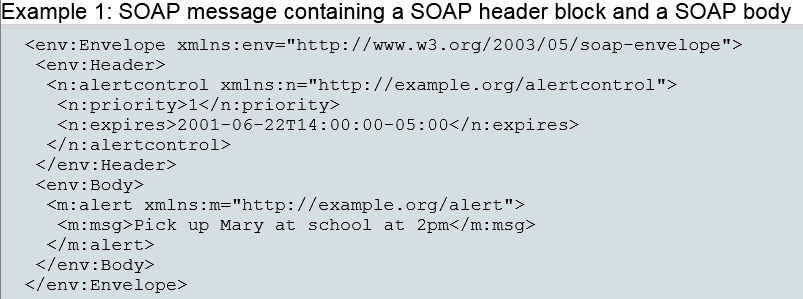
\includegraphics[width=\linewidth]{soap-msg-example}
	\caption{Příklad SOAP zprávy}
	\label{fig:soap-msg-example}
\end{figure}

Základní komunikační jednotkou v SOAP je zpráva, která je předávána mezi komunikujícími uzly. Obsah zprávy, který je zapouzdřený v takzvané obálce, se skládá z hlaviček a těla zprávy. Obrázek \ref{fig:soap-msg-example}, převzatý ze specifikace protokolu, znázorňuje příklad SOAP zprávy. V návaznosti na komunikační vzor RPC jsou SOAP zprávy mezi službami typicky používány k předání detailů o proceduře, jež má být vykonána, včetně vstupních parametrů. Výsledky těchto operací jsou vráceny v obdobném formátu.

% spojení WSDL služeb a SOAP
Použití protokolu SOAP jako formátu dat nad konkrétním komunikačním protokolem je definováno souborem pravidel, jež se nazývá SOAP Protocol Binding Framework. Tato pravidla popisují především detaily použití komunikačního protokolu pro předávání SOAP zpráv, dodržení kontraktu a zpracování případných chyb. V kontextu mé práce je důležité zejména napojení SOAP na HTTP u služeb popsaných WSDL dokumentem.

SOAP zprávy jsou skrze HTTP, vzhledem ke svému rozsahu, primárně přenášeny metodou POST a v rámci této práce je předpokládáno, že webové služby používající SOAP akceptují volání pouze s metodou POST. V dokumentu WSDL je propojení SOAP s HTTP definováno v elementu \verb|<binding>| a příklad takového propojení je uveden na obrázku \ref{fig:soap-http-binding}.

\begin{figure}[h]
	\centering
	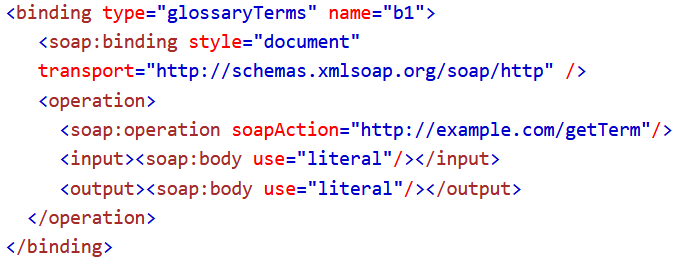
\includegraphics[width=11cm]{soap-http-binding}
	\caption{Propojení SOAP s HTTP v dokumentu WSDL}
	\label{fig:soap-http-binding}
\end{figure}


\section{REST}
\label{sec:rest}

%
% - co je REST
% - jak se liší od WS definované v předchozí sekci
% - základní popis elementů použitých v REST

Representational State Transfer (dále jen REST) je architektonický styl tvorby webových služeb, který ve své disertační práci \cite{fielding2000rest} popsal R. T. Fielding. Služby tvořené v tomto stylu se od služeb definovaných konsorciem W3C liší zejména využitím protokolu HTTP pro sémantiku aplikace a vyznačuje se také absencí stavu. 

R.T Fielding definoval styl REST skrze množinu omezení, jež jsou aplikována na systém vzájemně komunikujících komponent, což jsou v rámci této práce webové služby. Vybraná omezení jsou popsána v následujících odstavcích.

\subsubsection{Klient-server}
Důvodem pro toto omezení je princip oddělení zodpovědnosti klienta (např. uživatelského rozhraní) od serveru, čímž je umožněn nezávislý vývoj  obou stran.

\subsubsection{Absence stavu}

Omezení se týká zejména volání služby, jež musí obsahovat vše nutné pro jeho zpracování a není možné využít kontext uložený na straně serveru. Ten je tedy uložený na straně klienta a je proto nutná kontrola jeho konzistence při zpracování volání. Mezi výhody plynoucí z tohoto omezení patří zlepšení spolehlivosti a zpřehlednění komunikace.

\subsubsection{Uniformní rozhraní}

Komponenty vzájemně komunikují přes jednotné rozhraní, které odděluje jejich funkcionalitu od implementace. Rozhraní REST komponenty se vyznačuje čtyřmi vlastnostmi: identifikace zdrojů, manipulace jimi skrze reprezentace, sebe-popisující zprávy a hypermediální řízení (viz sekce \ref{sec:restful}).

\subsubsection{Vrstvený styl}
Komponenty jsou rozděleny do vrstev a každá z nich komunikuje pouze s komponentami v sousedních vrstvách. Aplikací tohoto modelu by mělo být dosaženo omezení komplexity a větší nezávislosti jednotlivých vrstev, respektive komponent v nich.

\subsection{Zdroj a jeho reprezentace}
\label{sec:rest-basics}

Na rozdíl od služeb vycházejících z RPC, jež jsou koncipovány jako množiny různých operací, jsou REST služby orientovány kolem zdrojů a manipulaci s jejich reprezentacemi. Architektura vycházející z toho stylu se nazývá ROA\footnote{Resource Oriented Architecture} a ve své publikaci\cite{restfulWebServices} ji popsal L. Richardson. Tato sekce se zabývá významem zdroje a jeho reprezentací v REST.

Zdroj (anglicky \textit{resource}) je klíčovou abstrakcí informace v REST a může představovat jakoukoliv pojmenovatelnou informaci jako například dokument, obrázek, webovou službu, nebo  kolekci jiných zdrojů. R. T. Fielding ve své práci\cite{fielding2000rest} definuje zdroj $R$ jako: 

\begin{quote}
	funkci $M_R(t)$, která pro čas $t$ vrací množinu ekvivalentních entit. Tato množina může být prázdná, nebo obsahovat reprezentace daného \textit{resource}, případně jeho identifikátory
\end{quote}

Pojem zdroj tedy neoznačuje konkrétní objekt nebo data, ale abstraktní koncept, který je konkrétním objektem nebo daty pouze reprezentován. Jako příklad lze uvést systém pro správu verzí, kde identifikátor 'poslední verze' označuje zdroj a samotná verze (0.8, 0.9, ...) jeho reprezentaci, která se s časem mění. Reprezentace různých zdrojů se mohou shodovat. V návaznosti na předchozí příklad by zdroje identifikované 'poslední verze' a 'verze 0.8' mohly být v určitý čas $t$ reprezentovány stejnou verzí '0.8'. 

Každý zdroj má alespoň jeden identifikátor, v případě Webu se jedná o URI. Tento identifikátor by měl být co nejvíce popisný a v rámci jedné služby dodržovat stejný styl\cite{restfulWebServices}. 

S reprezentacemi zdrojů je manipulováno HTTP voláním jejich identifikátorů (tedy URI) s nastavenou HTTP metodou, jež byly popsané v části \ref{sec:ws-tech}.

\subsection{RESTful služba}
\label{sec:restful}

Jedním z primárních účelů webových služeb založených na stylu REST je manipulace s XML reprezentacemi zdrojů pomocí jednotné množiny bezestavých operací, jimiž typicky jsou  \textit{create}, \textit{retrieve}, \textit{update} a \textit{delete}\cite{w3cWsArch}. Míra, kterou jednotlivé služby dodržují styl REST se různí a pojem 'RESTful' označuje ty, jež se REST drží nejvíce. Model zabývající se 'RESTful vyspělostí' dané služby byl představen L. Richardsonem a nazývá se Richardson Maturity Model. M. Fowler jej vysvětluje ve svém online článku \cite{restfulMaturity}, který je hlavním zdrojem informací pro následující odstavce. Model, uvedený na obrázku \ref{fig:rmm}, definuje čtyři níže popsané úrovně a pokud tyto služba splňuje, je označena jako RESTful (plně RESTová).

\begin{figure}[h]
	\centering
	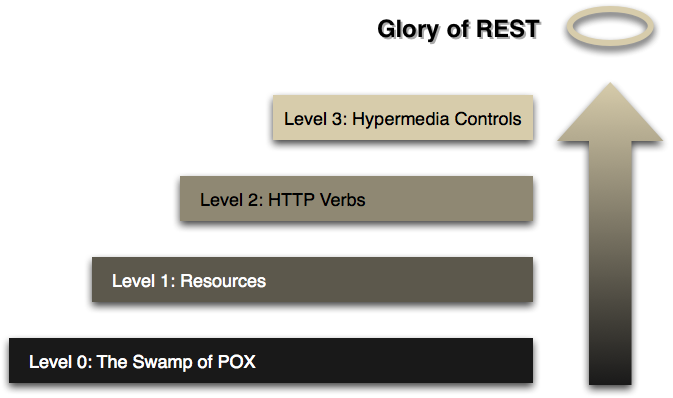
\includegraphics[width=9cm]{richardsonMaturityModel}
	\caption{Ilustrace Richardsonova modelu vyspělosti}
	\label{fig:rmm}
\end{figure}


\subsubsection{0. úroveň}
Služby v 0. úrovni se vyznačují použitím protokolu HTTP pro komunikaci, ale implementují vlastní sémantiku interakce, jež je typicky podobná stylu RPC. Služba je tedy například tvořena endpointem \textit{bookingService} a na tento jsou směřovány všechny volání obsahující informace o tom, co má služba vykonat. 

\subsubsection{Zdroje}
1. úroveň zavádí do služby zdroje, tak jak byly popsány v sekci \ref{sec:rest-basics}. Místo volání jednoho univerzálního endpointu služby jsou nyní volány endpointy jednotlivých zdrojů.

\subsubsection{HTTP metody}
Předchozí úrovně používají HTTP metody nezávisle na jejich účelu. Endpoint každého zdroje z předchozí úrovně by tedy například očekával volání POST i když by pouze vracel data. 2. úroveň tento přístup mění a služby používají HTTP metody tak, jak jsou v HTTP definované. Volání GET endpointu zdroje tedy vrací data, zatímco POST zdroj vytváří, nebo mění. 

\subsubsection{Hypermediální řízení}
Poslední úroveň zavádí princip HATEOAS\footnote{Hypertext As The Engine Of Application State}, ve kterém je klientovi s reprezentacemi zdrojů navíc předána informace o další možné manipulaci s nimi. Tím je docíleno většího oddělení klienta od poskytovatele, neboť server může mimo jiné měnit část schématu URI zdrojů a nenarušit tím schéma používané klientem.

\subsection{Verzování REST služeb}

Webové služby dodržující poslední úroveň Richardsonova modelu by za předpokladu statických vstupních bodů nemusely svou verzi vystavovat. Nicméně existuje nezanedbatelná část, jež na tuto úroveň nedosahují a tedy udržují statické rozhraní pro každou verzi, protože jakákoliv změna v schématu URI se negativně projeví na straně klienta. Ten totiž díky absenci HATEOAS nemůže tuto změnu dynamicky nijak zjistit je proto odkázaný na rozhraní služby. 

Může tedy nastat případ kdy poskytovatel v zájmu udržení zpětné kompatibility udržuje více verzí jedné služby současně. Existují různé způsoby jak vystavit konkrétní verzi, jedním z nich je uvedení verze v URI zdroje. Jedná se o běžnou a snadno implementovatelnou praktiku \cite{restApiVersion}\cite{restfulWebServices}. Dopady použití této praktiky na mou práci jsou rozebrány v částech \ref{sec:api-index} a \ref{sec:api-path-version}.


\section{Formální popis rozhraní webových služeb}
\label{sec:api-description-formats}

Aby bylo možné se službami komunikovat, je nutné znát jimi poskytované operace, zdroje a akceptovaný formát dat. Tyto informace jsou zahrnuté v rozhraní služby, jež může být popsáno různými způsoby s proměnlivou úrovní detailu. Služby popsané v části \ref{sec:rpc-ws} takové rozhraní automaticky poskytují ve strojově čitelné podobě, čímž mimo jiné umožňují automaticky generovat klienta a kostru serverové aplikace. V případě REST služeb (část \ref{sec:rest}) je situace složitější, protože univerzální standardizovaná podoba rozhraní neexistuje a to pak může mít podobu například Word dokumentu, nebo emailové konverzace. Výsledkem snah řešit problém se standardizací popisu rozhraní REST služeb jsou například strojově čitelné formáty Swagger\footnote{https://swagger.io/}, OpenApi\footnote{https://www.openapis.org/} nebo Raml\footnote{https://raml.org/}. 

Jak bude popsáno v kapitole \ref{sec:crce}, systém CRCE, pro který byl vyvíjen rozšiřující modul, jež je předmětem této práce, je v současnosti schopný indexovat webové služby pouze na základě implementace nebo popisu JSON-WSP, WADL a WSDL. Z tohoto důvodu zde jsou popsány pouze zmíněné podporované formáty.

\subsection{WSDL}

Formát WSDL je využíván převážně pro popis webových služeb využívajících protokol SOAP k výměně dat, nicméně od verze 2.0 lze popsat i REST služby. Formát současně existuje ve verzích 1.1 a 2.0. Z důvodů stáří verze 1.1, jež byla publikována v roce 2001, je tento popis zaměřen především na verzi 2.0. 

WSDL je formát založený na XML popisující webové služby jako množiny endpointů operujících nad zprávami (\textit{messages}), jež obsahují buď dokumentově, nebo procedurálně orientované informace. Abstraktně popsané operace a zprávy jsou spojeny s konkrétním síťovým protokolem a formátem zpráv, čímž je definován endpoint. Související endpointy jsou sdruženy do \textit{services} \cite{wsdl2}. Tabulka \ref{tab:wsdl-elements} obsahuje popis vybraných elementů použitých ve formátu WSDL 2.0.

\begin{table}[h]
	\centering
	\begin{tabular}{|l|c|}
		\hline
		Název & Popis \\
		\hline
		\hline
		service & Kolekce endpointů, na kterých je služba dostupná \\
		\hline
		endpoint & Detaily endpointu, na kterém je služba dostupná \\
		\hline
		message & Definice dat, jež jsou předmětem komunikace \\
		\hline
		portType & Množina operací služby \\		
		\hline
		operation & Implementační detaily konkrétní operace \\
		\hline
		binding & Implementační detaily nezbytné k přístupu ke službě \\
		\hline
		types & Definice vlastních typů \\
		\hline
		
	\end{tabular}
	\caption{Výběr elementů pro formát WSDL 2.0}
	\label{tab:wsdl-elements} 
\end{table}
 
\subsection{WADL}

WADL je strojově čitelný formát, jehož hlavním účelem je popis webových služeb založených na HTTP (například REST). Formát vznikl jako pokus o standardizaci popisu webových služeb, které jsou typicky popsané nestandardní, případě vzájemně odlišnou textovou dokumentací\cite{wadlSpec}.

Formát je založený na XML a popisuje webové služby jako kolekce zdrojů, nad kterými definuje operace (\textit{methods}). Zdroje \textit{resource} je možné vnořovat a každý zdroj je identifikován URI sestaveným podle předem daného vzoru. Tabulka \ref{tab:wadl-elements} obsahuje popis několika vybraných elementů, použitých k popisu webové služby.

\begin{table}[h]
	\centering
	\begin{tabular}{|l|c|}
		\hline
		Název & Popis \\
		\hline
		\hline
		resources & Kolekce zdrojů poskytovaných službou \\
		\hline
		resource & Popis konkrétního zdroje \\
		\hline
		method & Popis operace, která může být nad zdrojem provedena \\
		\hline
	\end{tabular}
	\caption{Výběr elementů pro formát WADL}
	\label{tab:wadl-elements} 
\end{table}
 
\subsection{JSON-WSP}

Formát JSON-WSP je založený na JSON a vychází z JSON-RPC, což je protokol pro vzdálené volání procedur. JSON-WSP popisuje rozhraní webových aplikací a i když měl původně nahradit JSON-RPC, je zatím ve stavu neformálního návrhu a není nijak standardizovaný ani neexistuje RFC s jeho specifikací nebo JSON schéma. Neoficiální specifikace je udržována na Wikipedii\cite{jsonWspSpec}.


JSON-WSP definuje službu pomocí objektů \textit{description}, \textit{request}, \textit{response} a \textit{fault}. Objekt \textit{description} popisuje rozhraní služby, obsahuje mimo jiné název služby, URL služby a kolekci metod, které služba dokáže vykonat. Objekty \textit{request}, \textit{response} a \textit{fault} definují podobu dat, které služba přijímá, respektive vrací. Tabulka \ref{tab:jsonwsp-elements} uvádí výběr objektů definovaných v \textit{description} relevantních pro mou práci.

\begin{table}[h]
	\centering
	\begin{tabular}{|l|c|}
		\hline
		Název & Popis \\
		\hline
		\hline
		methods & Kolekce metod vykonávaných službou \\
		\hline
		method & Popis konkrétní metody včetně parametrů a návratového typu \\
		\hline
		types & Definice vlastních typů \\
		\hline
	\end{tabular}
	\caption{Výběr elementů pro formát WADL}
	\label{tab:jsonwsp-elements} 
\end{table}
 
 
\chapter{Datové typy a porovnávání}

Tato kapitola rozebírá vlastnosti datových typů se zaměřením na jejich vzájemné porovnání. V první části kapitoly jsou představeny datové typy obecně, včetně jejich rozdělení v imperativní jazycích. Druhá část kapitoly se zabývá typovými systémy, způsoby kontroly typů a porovnáním datových typů. Vzhledem ke kontextu práce je text kapitoly zaměřen na staticky typované jazyky a typové systémy jazyků Java a XSD.

\section{Datové typy a jejich reprezentace}

TODO: formulace

Datový typ představuje množinu hodnot, ze které může proměnná, konstanta, funkce, nebo jiný výraz vzít svou hodnotu \cite{dataType}. O programovacích jazycích mluvíme jako o explicitně typovaných, pokud je název datového typu součástí syntaxe. Je-li navíc typová kontrola prováděna v čase překladu nazývají se tyto staticky typované \cite{cardelli2004}. Takovými jazyky jsou například C nebo Java.

Datové typy lze rozdělit na primitivní a složené. Ty lze dále dělit na záznamy a objektové typy.

 - datové typy se dělí podle něčeho na primitivní a složené
 - složené datové typy se navíc dělí na záznamy a objekty
 - všechny tyto jsou popsány v následujících sekcích
 
\subsection{Primitivní datové typy}
 
  - nejzákladnější datové typy jazyka
  - na rozdíl od objektových datových typů zde neexistuje dědičnost
  - používané k reprezentaci základních datových jednotek: číslo, znak, pravdivostní hodnota
  - říkají kompilátoru, nebo interpretu co konkrétní data v paměti reprezentují
  - Java má 8 primitivních datových typů
  - Příklady primitivních datových typů jazyka Java 8 v tabulce \ref{tab:java-prim-types}
 
\begin{table}[h]
	\centering
	\begin{tabular}{|l|c|}
		\hline
		Název datového typu & Rozsah hodnot \\
		\hline
		\hline
		int & $<-2^{31};2^{31}-1>$ \\
		\hline
		boolean & true, false \\
		\hline
		char & 16-bit Unicode znaky \\
		\hline
	\end{tabular}
	\caption{Výběr primitivních datových typů jazyka Java}
	\label{tab:java-prim-types}
\end{table}

\subsection{Záznamy}

Datový typ záznam (anglicky \textit{record}) je kolekcí položek různých datových typů s typicky pevně daným pořadím \cite{felleisen2001}. Příkladem záznamu v jazycích je například \textit{struct} v C \textit{record} v Pascalu. Jazyk Java datový typ záznam nedefinuje.

Jako na záznam se také dá nahlížet na vlastní datový typ definovaný v XSD elementem \textit{complexType}, jež představuje pojmenovaný výčet položek s různými datovými typy. Pro srovnání je na obrázku \ref{fig:record-xsd-c} uveden příklad záznamu \textit{personinfo} definovaného pomocí \textit{complexType} v XSD a \textit{struct} v C.

\begin{figure}[h]
	\centering
	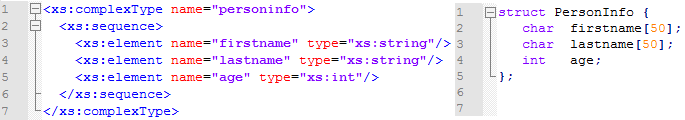
\includegraphics[width=\linewidth]{record-example}
	\caption{Záznam v XSD a C}
	\label{fig:record-xsd-c}
\end{figure}
 

\subsection{Objektové datové typy}

 - datový typ složený z dat a metod
 - šablona objektového datového typu se v Jave nazývá třída (\textit{class})
 - podpora dědičnosti, polymorfismu
 - v Jave také rozhraní 
 - zmínit self
 

\section{Typový systém}

- úzce souvisí s návrhem jazyka
- definice typového systému podle \cite{pierce2002}:

\begin{quote}
A type system is a tractable syntactic method for proving the absence of
certain program behaviors by classifying phrases according to the kinds
of values they compute.
\end{quote}

\begin{quote}
	Typový systém je sledovatelná syntaktická metoda pro prokázání absence určitých chování programu klasifikováním frází podle druhů hodnot, které představují.
\end{quote}

- Typový systém udává pravidla pro kontrolu typů v programovacím jazyce nezávisle na konkrétních algoritmech. Jeho primárním účelem je zabránění výskytu chyb za běhu programu\cite{cardelli2004}.
- elementární jazyk s podporou typů: simply typed lambda calculus
- lambda kalkul je vhodným nástrojem k definici pravidel typového systému

- přednášky z FJP
- něco od datových typech obecně: https://www.cs.cmu.edu/~rwh/introsml/core/datatypes.htm
- jak jazyky řeší datové typy
	- rekurzivní vs. nerekurzivní
- něco od taových typech obecně: https://www.cs.cmu.edu/~rwh/introsml/core/datatypes.htm

\subsection{Rekurzivní datové typy}

- možná fajn na rekurzivní typy: http://web.mit.edu/6.005/www/sp16/classes/16-recursive-data-types/recursive/
- převzato z \cite{pierce2002}
- typickým příkladem je immutable seznam
	- seznam List<T> je buď prázdný, nebo je tvořený dvojicí first:T a rest:List<T>
	- jeho konstruktor má tvar List(T, List<T>)
- problém spočívá v rekurzivním rozvoji, protože pravá strana je definována tím, co se snažíme definovat
- to vede na nekonečný strom
- přístup k řešení se dělí podle toho, jak je vyřešen první krok rekurzivního rozvoje
	- equi-recursive
		- definitionally equal = zaměnitelné v jakémkoliv kontextu, protože představují stejné nekonečné stromy
	- iso-recursive
		- rekurzivní rozvoj = 1. krok celého rozvoje
		- jazyk musí mít operace fold() a unfold()
		- ty jsou navzájem isomorfní

\subsection{Typový systém XSD}

 - pouze primitivní typy nebo záznamy
 - definováno XML
 - dědičnost: https://www.liquid-technologies.com/xml-schema-tutorial/xsd-extending-types

\subsection{Typový systém jazyka Java}

 - primitivní typy nebo objekty
 - abstraktní třídy, rozhraní, dědičnost

\section{Typová kontrola}

- jak to funguje
- problémy při porovnání
- většina informací v této části založena na publikace B. C. Pierce \cite{pierce2002}.
- k typové kontrole jsou použity dvě relace: matching a subtyping

Rozeznáváme dva druhy typové kontroly:

\paragraph{Statická typová kontrola} probíhá v čase překladu a konkrétní datové typy proměnných jsou známé ještě před spuštěním programu. V případě detekce typovací chyby dojde k přerušení překladu a sestavení programu, čímž je zabráněno případným chybám, které by mohly vést k pádu programu za běhu.

\paragraph{Dynamická typová kontrola} probíhá za běhu programu a provádí ji například interpret jazyka. Oproti statické typové kontrole umožňuje tato spuštění programů s chybami v typech (například \verb|int a = 1 + "abc"|), jež se mohou projevit zastavením nebo pádem programu.

- většina jazyku používající statickou kontrolu používá i dynamickou, kvůli meta-programování, downcastingu, atp

- relace jež se zabývá vztahem mezi typy a která se používá k vyhodnocení typové bezpečnosti se nazývá subtyping a je popsána v následující sekci



\subsection{Subtyping}
\label{sec:subtyping}

- binární relace definovaná nad typy
- reflexivní A <: A
- tranzitivní A <: B, B <: C => A <: C
- značení A <: B čteme jako A je sub-typ B
- znamená to, že A může být použito kdekoliv, kde je očekáváno B
- příklad: \textit{java.lang.Long} je sub-typ \textit{java.lang.Number}, protože typ \textit{Long} může být použit kdekoliv tam, kde je očekáván typ \textit{Number} 

\subsubsection{Primitivní typy}

V případě primitivních typů subtyping označuje schopnost jednoho typu pojmout jiný. Tedy například primitivní typ \textit{double} je schopný reprezentovat všechna čísla z \textit{float} (ale ne naopak) a proto platí $float <: double$. V případě datových typů pro celá čísla v Jave pak platí následující:

\begin{figure}[h]
	\centering
	$byte <: short <: int <: long$
\end{figure}

\subsubsection{Záznamy}

Relace subtypingu je pro záznamové datové typy $S = \{k_1:S_1 ... k_m:S_m\}$ a $T = \{l_1:T_1 ... l_n:T_n\}$ je definována pomocí následujících třech kritérií:

\begin{itemize}
	\item \textbf{subtyping do šířky}: Delší záznam je sub-typ kratšího záznamu ($n \le m$),
	\item \textbf{subtyping do hloubky}: Všechny položky na stejné pozici musí být v relaci subtypingu (pro každé $i : S_i <: T_i$),
	\item \textbf{permutační subtyping}: Na pořadí položek nezáleží, pokud existuje $\{k_j:S_j | j \in 1..n \}$, které je permutací $\{l_i:T_i | i \in 1..n \}$.
\end{itemize}

Uvažujeme-li na příklad typy $S$ a $T$ definované jako:

\begin{equation}
\centering
	S = \{a:int, b:boolean, c:char\}, \quad
	T = \{a:long\}
\end{equation}

 platí, že $S <: T$, protože $S$ má méně položek, než $T$ a zároveň $int <: long$. 
 
 V případě typů $S$ a $T$ definovaných jako:
 
\begin{equation}
	\centering
	S = \{a:int, b:boolean, c:char\}, \quad
	 T = \{a:short, b:char\}
\end{equation} 

 $S <: T$ neplatí, protože $\overline{int <: short}$ a $\overline{boolean <: char}$ a i když je dodrženo pravidlo "do šířky", není dodrženo pravidlo "do hloubky" ani v případě použití permutačního pravidla.

\subsubsection{Funkce}

Relaci subtypingu lze také definovat pro funkce. Zde se vychází z předpokladu, že funkci lze předat jako parametr a je tedy nutné určit, zda je možné použít typovanou funkci v kontextu, kde je očekáván jiný typ. 

Uvažujeme-li funkce $f_1$ a $f_2$ definované v \ref{eq:functions}, pak relace subtypingu platí pokud jsou splněny podmínky $T_1 <: S_1$ a $S_2 <: T_2$ (viz \ref{eq:function-subtyping}).

\begin{equation}
	f_1: S_1 \rightarrow S_2,\quad f_2: T_1 \rightarrow T_2
	\label{eq:functions}
\end{equation}

\begin{equation}
	T_1 <: S_1, S_2 <: T_2 \vdash f_1 <: f_2
	\label{eq:function-subtyping}
\end{equation}

V případě typů na levé straně funkce (typy vstupních parametrů) je relace subtypingu kontravariantní. Tato změna má následující zdůvodnění: pokud je někde očekávána funkce s argumentem typovaným na $T_1$, je bezpečné použít funkci s argumentem typovaným na $S_1$ tak, že $T_1 <: S_1$, protože $T_1$ lze použít tam, kde je očekáváno $S_1$ (definice subtypingu). 

Očekáváme-li v programu například funkci $f_1: short \rightarrow double$, je bezpečné ji nahradit funkcí $f_2: int \rightarrow float$, protože datový typ \textit{int} dokáže pojmout typ \textit{short}, který by při volání funkce byl použitý. Výsledek vrácený funkcí $f_2$ je typovaný na \textit{float} a je tedy bezpečné jej uložit do proměnné typované na \textit{double}, což je očekávaný návratový typ $f_1$. Obě podmínky z \ref{eq:function-subtyping} jsou tedy splněné a platí $f_2 <: f_1$.

\subsubsection{Objekty} 	

Z pohledu subytypingu se na objektové datové typy dá nahlížet jako na záznam s přidanými funkcemi. Dva objektové typy jsou v relaci subtypingu pokud jsou v této relaci i všechny jejich proměnné a metody\cite{abadi1995subytping}. 

Problém s relací subtypingu nastává v případě rekurzivních typů s funkcemi jejichž argumentem je \textit{self} a výstupem je hodnota typovaná stejně jako \textit{self}, tedy například typ $X$ s funkcí $f: X \rightarrow X$. Příčinou je nedodržení principu kontravariance popsaného u subtypingu funkcí. Následující příklad, který tento problém ilustruje, byl přejat z \cite{abadi1995subytping} a pro vyjádření typů používá upravenou notaci lambda kalkulu, která označuje funkce symbolem $^+$. 

Uvažujeme-li typy $Max$, $MinMax$ definované v \ref{eq:max-class} a \ref{eq:minmax-class}, pak při konstrukci relace $MinMax <: Max$ narazíme na funkce $max^+: Max \rightarrow Max$ a $max^+: MinMax \rightarrow MinMax$. Aby mezi těmito byla relace subtypingu, musí zároveň platit $Max <: MinMax$ a $MinMax <: Max$ což je spor a typ $MinMax$ tedy není pod-typ $Max$. Řešení tohoto problému je stručně popsáno v následující části.

\begin{equation}
	Max \triangleq \mu(X)[n:Int, max^+:X\rightarrow X] 
	\label{eq:max-class}
\end{equation} 
\begin{equation}
	MinMax \triangleq \mu(Y)[n:Int, max^+:Y\rightarrow Y, min^+: Y \rightarrow Y] 	
	\label{eq:minmax-class}
\end{equation}

\subsection{Matching na základě subtypingu}

Relace subtypingu v případě rekurzivních objektových typů naráží na problém popsaný v sekci \ref{sec:subtyping}. M. Abadi a L. Cardeli ve svém článku \cite{abadi1995subytping} zavádějí relaci \textit{matching} nad tzv. protokoly typů, což jsou reprezentace jejich rozhraní. Tato relace vychází ze subtypingu a je zapisována jako \textit{A <\# B}, což znamená "protokol typu A rozšiřuje protokol typu B". 

V příkladu z předešlé sekce \ref{sec:subtyping} by protokoly typů $Min$ a $MinMax$ byly definovány jako:

\begin{equation}
	MaxProt \triangleq n:Int, max^+: Self \rightarrow Self
\end{equation}
\begin{equation}
	MinMaxProt \triangleq n:Int, max^+: Self \rightarrow Self, min^+: Self \rightarrow Self
\end{equation}

Klíčové slovo \textit{Self} označuje typ, pro který mimo jiné platí $Self <: Self$. Pokud použijeme postup konstrukce subtypingu na zmíněné protokoly, výsledkem bude \textit{MinMaxProt <\# MaxProt}. Relace matching nad protokoly typů neimplikuje subtyping daných typů a nelže tedy vyvodit, že $MinMax <: Max$.


\chapter{Získávání metadat webových služeb v CRCE}
\label{sec:crce}

Cílem této práce je vytvořit rozšíření pro úložiště CRCE\footnote{Component Repository supporting Compatibility Evaluation}, které bude schopno vyhodnocovat vzájemnou kompatibilitu indexovaných webových služeb. Tato kapitola představuje samotné úložiště, formát metadat a obecný způsob jejich získání. Na konci kapitoly je popsán princip fungování konkrétních rozšíření, která indexují webové služby (tzv. indexery).

\section{CRCE}

CRCE je komponentové úložiště dlouhodobě vyvíjené a spravované výzkumnou skupinou ReliSA na Katedře Informatiky ZČU, jehož primárním účelem je indexace a následná kontrola vzájemné kompatibility komponent. Úložiště je postaveno na modulární architektuře (viz obrázek \ref{fig:crce-arch}) a je tedy možné přidat rozšíření pro indexaci a zpracování vlastních dat.

\begin{figure}[h]
	\centering
	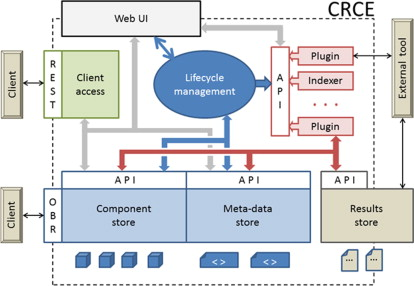
\includegraphics[width=10cm]{crce-arch.jpg}
	\caption{Architektura CRCE}
	\label{fig:crce-arch}
\end{figure} 

\subsection{Metadata komponent}
\label{subsec:crce-metadata}

Data, která vzniknou indexací komponenty a případným dalším zpracováním (např. porovnáním) jsou uložena do souboru metadat a představují klíčový element systému CRCE. Návrh struktury  těchto metadat, který je naznačen na obrázku \ref{fig:crce-resource-uml}, vychází z konceptu OBR\footnote{OSGi bundle repository} jehož základními entitami jsou mimo jiné \textit{Resource}, \textit{requirements} a \textit{capabilities}\cite{brada2015repository}. 

Entita \textit{Resource} reprezentuje komponentu uloženou v CRCE, \textit{requirements} a \textit{capabilities} jsou množiny vlastností, popisující co komponenta ke své správné funkci vyžaduje, respektive co naopak poskytuje. Model také umožňuje přidání key-value atributů k jednotlivým vlastnostem a jejich detailům.
 
 \begin{figure}[h]
 	\centering
 	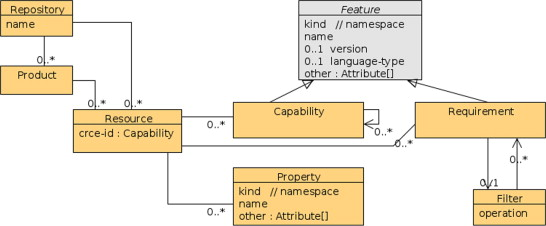
\includegraphics{resource-uml}
 	\caption{Reprezentace metadat v CRCE}
 	\label{fig:crce-resource-uml}
 \end{figure}

V mé práci jsem pracoval především s poskytovanými vlastnostmi (množina \textit{capabilities}) a proto zde popíši hlavně jejich strukturu. Každá konkrétní vlastnost je reprezentována elementem \textit{Capability} a od ostatních je odlišena identifikátorem \textit{namespace}. Detaily konkrétní vlastnosti jsou popsány elementy \textit{Property} a \textit{Attribute}, kde \textit{Property} reprezentuje logický celek několika atributů. Například parametr endpointu REST služby shlukuje atributy popisující jeho jméno, datový typ atp. \textit{Attribute} pak představuje pár klíč-hodnota, který nese konkrétní informace jako např. jméno endpointu, nebo datový typ parametru.

Z obrázku \ref{fig:crce-resource-uml} je vidět rekurzivní povaha elementu \textit{Capability}, čehož je využito ke skládání jednodušších vlastností do složitějších celků. Vznikne tím stromová struktura, která je vhodná k modelování hierarchických dat mezi něž patří například popisy webových služeb. V případě takto komplexních vlastností je ke komponentně (\textit{Resource}) přiřazena pouze jedna, tzv. kořenová, \textit{Capability}, která reprezentuje celou vlastnost.

%Metadata v CRCE mají hierachickou strukturu:
%- Resource + Capability + Properties + Atributy
%- taky Requirements, ale ty v práci nepoužívám
%- Resource reprezentuje indexovanou komponentu
%- jednotlivé featury (indexovaná data) jsou reprezantovány stromem Capabilit
%- k Resource je vždy přiřazena root Capabilita
%- každá Capabilita má namespace, podle kterého lze určit co za konkrétní vlastnost popisuje
%- v případě root Capability by namespace měl být unikátní pro Resource (a resource by tedy neměl mít více root Capabilit s jedním namespace (snad?))
%- detaily fetatury jsou pak uloženy v dětských capabilitách, jejich Properties a Attributes
%- Capability mají Attributy + Properties
%- Properties mají atributy
%- Attributes pak nesou konkrétní hodnoty (Capability a Propeties slouží pouze jako jakési kontejnery)
%- Lze tak modelovat různé vlastnosti indexovaného objektu (viz \cite{brada2015repository}, tam je to dobře popsaný)
%- hierarchická struktura metadat je vhodná pro reprezentaci webových API, která jsou rovněž hierarchická

\subsection{Životní cyklus komponenty v CRCE}

Úložiště bylo původně navrženo pro ukládání OSGi komponent, nicméně indexovat lze jakoukoliv komponentu. Komponenta je v CRCE popsána již zmíněnými metadaty a prochází vlastním životním cyklem naznačeným na obrázku \ref{fig:crce-comp-lc}.

\begin{figure}[h]
	\centering
	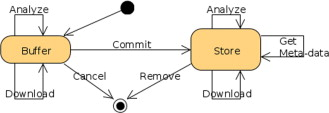
\includegraphics{crce-component-lc.jpg}
	\caption{Životní cyklus komponenty v CRCE}
	\label{fig:crce-comp-lc}
\end{figure} 

Životní cyklus má dvě hlavní fáze, jimiž jsou \textit{Buffer} a \textit{Store}. Komponenta po nahrání do úložiště nejprve prochází fází \textit{Buffer}, v níž dojde k indexaci obsahu, kontrole vnitřní konzistence a kompatibility komponenty. Pokud touto fází projde bez chyb, může uživatel pomocí operace \textit{commit} komponentu nahrát do trvalého úložiště, čímž dojde k přechodu  do fáze \textit{Store}.

V obou fázích jsou nad komponentou prováděny operace z nichž \textit{analyze} je nejvíce relevantní mé práci, protože právě během této operace dochází ke sběru metadat (fáze \textit{Buffer}) a dalším výpočtům nad nimi (fáze \textit{Store}). Modul s rozšířením, který je předmětem mé práce bude zařazen mezi výpočty prováděné nad metadaty během \textit{analyze}, kde bude vyhodnocovat vzájemnou kompatibilitu webových služeb. Způsoby sběru těchto metadat, ke kterým dochází ve fázi \textit{Store}, jsou popsány v následující sekci. 

%
%- primárně komponenta = OSGI bundle, ale může být cokoliv (např i pouhý textový soubor)
%
%- nahrání do bufferu
%
%- analýza
%
%- commit do store
%
%- další analýza
%
%- během toho se vytvářejí metadata
%
%- jednotlivé fáze mají callbacky, na které je možné v modulu navěsit vlastní funkcionalitu (\textit{BeforeUploadToBuffer}, \textit{AfterUploadToBuffer}, \textit{BeforeCommit}, ...)

\section{Indexování webových služeb}
\label{sec:api-index}

V této podkapitole je krátce popsán obecný způsob indexace komponent v CRCE. Následně je podrobněji rozebráno indexování webových služeb konkrétními moduly a reprezentace popisu API metadaty v CRCE. Na závěr jsou také uvedeny limity indexování.


\subsection{Obecná indexace komponenty}

Indexace komponenty a související sběr metadat je proveden ve fázi \textit{Buffer} k tomu určenými moduly. Ty jsou vzájemně nezávislé a obecně platí, že každý nich je zaměřen na sběr nějaké logicky ucelené části dat jako například informace o OSGi bundlu, maven koordináty, nebo popis webových služeb. Vlastní data komponenty zůstávají během tohoto procesu nezměněná což v kombinaci s řetězením indexerů zaručuje mimo snadnou rozšiřitelnost také transparentní přístup ke komponentě každému z nich. 

\subsection{Indexace komponenty s webovou službou}

Soubor obsahující implementaci, nebo popis API je v CRCE vnímán jako komponenta a prochází tedy zmíněným životním cyklem včetně výše popsané indexace. Pro popis webových služeb existuje mnoho standardních i nestandardních způsobů, jak již bylo zmíněno v kapitole \ref{sec:web-services-principles}. Z tohoto důvodu je není možné všechny analyzovat jedním indexerem a je nutné zaměřit se pouze na část z nich. 

V současné době tedy existují dva moduly podporující několik popisných formátů a implementací. Konkrétně se jedná o modul pro indexaci webových služeb založených na architektonickém stylu REST\cite{hessova2015rest} a o modul pro indexaci webových služeb s popisem ve formátu WSDL, WADL, nebo Json-WSP \cite{pejrimovsky2015ws}. Oba dva vznikly v rámci diplomových prací a jsou stručně popsány v následujících sekcích.

%- někde by asi bylo fajn ustanovit názvosloví použité v práci:
%\begin{itemize}
%	\item co je API: interface přístupné skrze síť (internet)
%	\item co je web service: service popsaný WSDL, WADL, nebo Json-WSP dokumentem
%	\item co je service: Service element in WSDL
%	\item co je endpoint
%	\item WSDL: port+operation
%	\item endpoint: REST, WADL, JSON-WSP
%\end{itemize}

\begin{figure}[h]
	\centering
	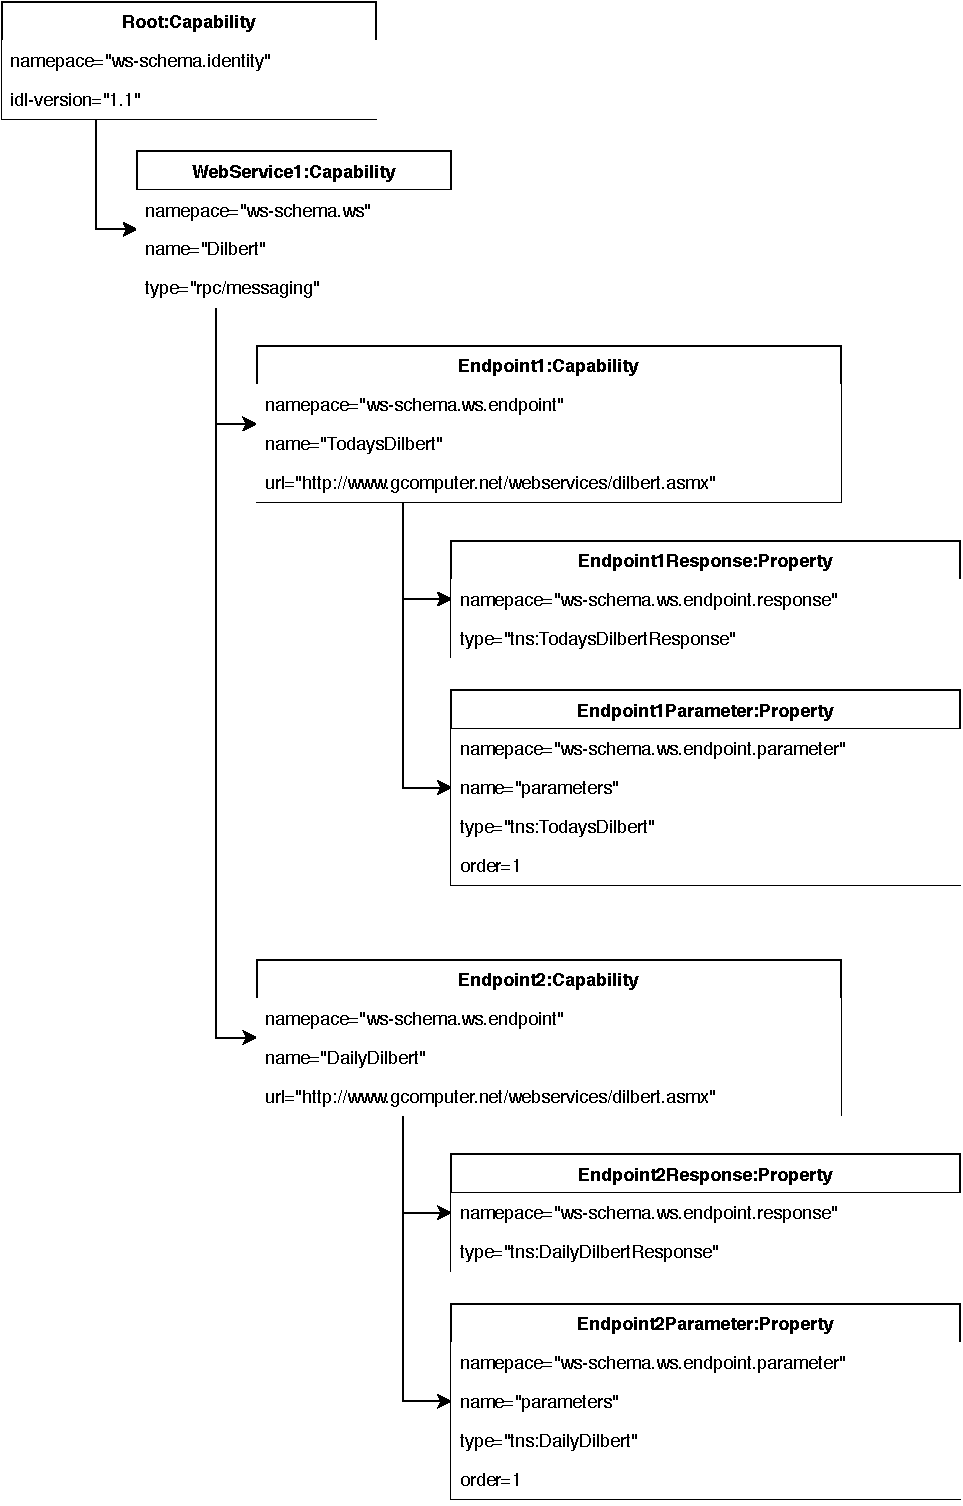
\includegraphics[height=11cm]{indexed-api-example}
	\caption{Příklad indexované SOAP webové služby pro komix Dilbert }
	\label{fig:indexed-api-example}
\end{figure}

\subsection{Struktura metadat popisující webovou službu}

Jak již bylo zmíněno v části \ref{subsec:crce-metadata}, hierarchickou strukturu popisu API lze vhodně vyjádřit metadaty CRCE. Během indexování komponenty reprezentující API jsou shromážděny různé typy popisných vlastností. Jedním z těchto typů je i samotný popis webové služby, který je reprezentován stromem metadat a ke komponentě je přiřazen skrze  kořenovou \textit{Capability}.   

I když jsou různé druhy API indexovány rozdílnými moduly, výsledná metadata mají podobnou strukturu. Příklad metadat API je zobrazen na objektovém diagramu \ref{fig:indexed-api-example}, jedná se o webovou službu, která vrací strip komixu Dilbert pro dnešní den.

Z uvedeného obrázku je vidět, že klíčové elementy API jako web service, nebo endpoint jsou reprezentovány objektem \textit{Capability}. Detaily těchto elementů jsou popsány objekty \textit{Property}. Jedná se zejména o parametry endpointů, těla requestů a response. Objekt \textit{Attribute} pak představuje konkrétní hodnoty, jež jsou na obrázku naznačeny jen jako páry "klíč=hodnota". \textit{Attribute} nemusí být vázaný jen na \textit{Property} a lze jej použít i pro popis \textit{Capability}, jak je tomu např. u objektu \textit{WebService1}.

\subsection{Indexování REST služeb}

Modul pro indexování REST API vznikl v rámci diplomové práce Bc. Gabriely Hessové. Princip sběru dat je založen na binární analýze java archivů (JAR) obsahujících implementaci REST služeb pomocí frameworků splňujících specifikaci JAX-RS a frameworku Spring Web MVC. Modul byl testován na frameworcích Jersey verze 2.26, RESTEasy verze 3.0.16 a  Spring Boot verze 1.5.9 \cite{hessova2015rest}.

Z implementace REST služby modul rekonstruuje kolekci endpointů s jejich parametry, tělem requestu, response a případnými parametry response. Každý endpoint je reprezentován entitou \textit{Capability}, všechny další jeho vlastnosti pak entitami \textit{Property}. Výčet všech indexovaných elementů rozhraní je uveden v tabulce \ref{tab:rest-indexed}.

\begin{table}[h]
	\centering
	\begin{tabular}{|l | c | c |}
		\hline
		Element API & Entita v metadatech & Vstaženo k\\
		\hline
		\hline
		Endpoint & Capability & - \\
		\hline
		Request body & Property & Endpoint \\
		\hline
		Request parameter & Property & Request \\
		\hline
		Response & Property Endpoint & Endpoint \\
		\hline
		Response parameter & Property & Response \\
		\hline
	\end{tabular}
	\caption{Seznam indexovaných elementů REST služby a jejich reprezentací v metadatech}
	\label{tab:rest-indexed}
\end{table}

\subsection{Indexování webových služeb na základě popisu}

Modul pro indexování webových služeb vznikl v rámci práce Bc. Davida Pejřimovského. Oproti předchozímu modulu pro indexaci REST služeb nepracuje tento s její implementací, ale s popisným souborem služby, tak jak bylo uvedeno v kapitole \ref{sec:web-services-principles}. Podporované formáty popisu služeb jsou WSDL (verze 1.1 i 2.0) pro SOAP webové služby, WADL a Json-WSP pro REST služby\cite{pejrimovsky2015ws}.

Struktura dat vytvořených pro REST služby (tedy z popisu WADL, nebo JSON-WSP) je podobná struktuře dat vytvořenou předchozím indexerem. Endpoint je tedy reprezentován entitou \textit{Capability}, jeho parametry entitami \textit{Property}. Z popisu Json-WSP je ještě vytvořena reprezentace response pro daný endpoint (entita \textit{Property}). Z popisu WADL se žádné další vlastnosti endpointů nezískávají.

Z WSDL popisu je vytvořena reprezentace služeb, jež jsou popsány xml elementy \verb|<wsdl:service>| a jejich vnořených endpointů. Endpoint je ve WSDL popsán elementem \verb|<wsdl:port>| a má definované operace (elementy \verb|<wsdl:operation>|), nicméně modul tyto nevnořuje a vytváří zjednodušenou reprezentaci. Model endpointu tedy obsahuje metadata získaná z elementů \verb|<wsdl:operation>| a url definovanou v elementu \verb|<wsdl:port>|. Služby i endpointy jsou v metadatech reprezentovány entitami \textit{Capability}. Oproti REST službám, které mají jednu úroveň vnoření \textit{Capability}, zde vznikají úrovně dvě. Výčet elementů API a jejich reprezentace v metadatech je uveden v tabulce \ref{tab:ws-indexed}.

\begin{table}[h]
	\centering
	\begin{tabular}{|l | c | c |}
		\hline
		Element API & Entita v metadatech & Vztaženo k \\
		\hline
		\hline
		Service & Capability & - \\
		\hline
		Endpoint & Capability & Service \\
		\hline
		Endpoint parameter & Property & Endpoint \\
		\hline
		Response & Property & Endpoint \\
		\hline
		Response parameter & Property & Endpoint \\
		\hline
	\end{tabular}
	\caption{Seznam indexovaných elementů webové služby a jejich reprezentací v metadatech}
	\label{tab:ws-indexed}
\end{table}

Logika parsování WSDL souborů (verze 1.1. i 2.0) obsahovala chybu ve čtení adresy endpointu. Ta byla očekávána v atributu \verb|action| elementu \verb|<wsdl:operation>|, který ale není uveden ve specifikaci WSDL 1.1 \cite{wsdl1} ani WSDL 2.0 \cite{wsdl2}. Tuto chybu jsem v rámci mé práce opravil.

\subsection{Limity indexování}
\label{sec:index-limits}

Současný proces indexování webových služeb naráží na dva známé problémy týkající se datových typů. Jedná se o indexování rekurzivních datových typů a absenci samotných definic typů.

První problém se týká zejména indexování webových služeb podle popisných souborů, protože ty definice typů obsahují. Způsoby rozvoje a ukládání datových typů jsou popsány v \cite{abadi1995subytping}, nicméně logika zatím není implementována. Druhý problém se týká binární analýzy REST služeb, protože archiv s implementací služby nemusí nutně obsahovat definice tříd. Ty mohou být například v jiném artefaktu, na který se archiv pouze odkazuje skrze závislost.

Z těchto důvodů je do metadat uložen pouze název datového typu což snižuje možnosti porovnávání služeb.

% - custom datové typy
% - 2 problémy
%	- rekurzivní typy
%		- jsou způsoby pro jejich rozvoj: \cite{abadi1995subytping} a % ukládání
%		- nicméně indexovací logika není implementovaná (ani v jednom ze zmíněných indexerů)
%	- chybějící definice custom typů
%		- v případě např REST jsou uloženy v implementaci (nemusí se jednat ani o stejnou knihovnu) a indexer k nim nemusí mít přístup
%		- tím pádem je jméno datového typu (např. fully qualified name v případě Java třídy) jedinou informací, která je o typu dostupná
% - oba dva moduly používají jiné identifikátory pro stejné elementy (endpoint, parametr, ...) proto nelze vzájemně porovnat REST indexovaný prvním a druhým modulem

\chapter{Porovnávání webových služeb}
\label{sec:alg}

Cílem této práce je rozšířit systém CRCE o funkcionalitu pro porovnání webových služeb. Tato kapitola detailně rozebírá porovnávací algoritmus společně s daty, nad kterými je možné porovnávač použít. Zároveň je zde popsán způsob vyhodnocení výsledků porovnání a formát uložení takto získaných dat.

\section{Reprezentace rozdílů a kompatibility}
\label{sec:diff-info}
Webové služby jsou popsány komplexní strukturou metadat, která byla uvedena v předchozí kapitole. Rozdíl mezi těmito strukturami lze vyjádřit pouhou pravdivostní hodnotou (stejné, nebo nestejné), nicméně takový přístup skrývá před klientem většinu informací, na základě kterých by se mohl rozhodnout o dalším postupu a tím značně snižuje použitelnost aplikace. Mimo to, samotná skutečnost, že metadata webových služeb se neshodují nemusí nutně z pohledu klienta znamenat nekompatibilitu. Z těchto důvodů je k reprezentaci rozdílů mezi službami třeba použít vhodnější metodu.

Článek \cite{brada2006diff} zabývající se možnostmi evaluace kompatibility komponent na základě relace subtypingu, nahlíží na komponentu skrze její rozhraní jako na datový typ a popisuje odlišnosti v různých úrovních stromu metadat (třída, operace, parametr, ...). Na základě těchto odlišností (a relace subtypingu) je pak určena míra kompatibility dvou komponent. Protože je webová služba v CRCE reprezentována komponentou a na její rozhraní se dá také nahlížet jako na kontrakt datového typu, je tento přístup vhodný k reprezentaci rozdílů mezi webovými službami. Oproti pouhé pravdivostní hodnotě je navíc klientovi poskytnuta detailní informace o konkrétních rozdílech mezi službami. Z těchto důvodů jsem se rozhodl použít výše zmíněný způsob reprezentace rozdílů v mé práci. 

Datové struktury použité pro reprezentaci rozdílů dvou entit a jejich vzájemné kompatibility navržené v rámci citovaného článku se nazývají \textit{Diff} a \textit{Compatiblity}. \textit{Diff} je definován jako rekurzivní typ, který uchovává jak konkrétní informace o rozdílu skrze podřazené \textit{Diff} tak i úroveň odlišnosti zvanou \textit{Difference}. Tyto úrovně jsou popsány tabulkou \ref{tab:diffs} a v citovaném článku tvoří obor hodnot funkce $diff(a,b): Type \times Type \rightarrow Difference$. Třída \textit{Compatibility} uchovává informace o kompatibilitě dvou komponent (reprezentovány entitami \textit{Resource}) společně s detaily jejich rozdílů, jež jsou reprezentovány stromem \textit{Diff}.

\begin{table}[h]
	\centering
	\begin{tabular}{|l|c|c|c|}
		\hline
		Název úrovně & Zkratka & Váha & Popis \\
		\hline
		\hline
		None & NON & 1 & $a = b$ \\
		\hline
		Insertion & INS & 2 & $a$ není definováno, ale $b$ ano \\
		\hline
		Deletion & DEL & 2 & $a$ je definováno, ale $b$ ne \\
		\hline
		Specialization & SPE & 3 & $b$ je subtyp $a$ ($b <: a$) \\
		\hline
		Generalization & GEN & 3& $a$ je subtyp $b$ ($a <: b$) \\
		\hline
		Mutation & MUT & 4 & kombinace \textit{INS}/\textit{SPE} a \textit{DEL}/\textit{GEN} \\
		\hline
		Unknown & UNK & 5 & $a$ nelze porovnat s $b$ \\
		\hline
	\end{tabular}
	\caption{Popis úrovní rozdílů}
	\label{tab:diffs}
\end{table} 

Způsob vyhodnocení rozdílů dvou webových služeb společně s významem jednotlivých úrovní \textit{Difference} a jejich vah pro klienta je popsán na konci této kapitoly. Pro přehlednost jsou jednotlivé úrovně rozdílů v průběhu kapitoly nazývané jejich zkratkami. 

%Popis výsledné datové struktury
%\begin{itemize}
%	\item Diff, Compatibility
%	\item vychází z \cite{brada2006diff}
%	\item stromová struktura rozdílů mezi jednotlivými uzly stromu metadat
%	\item obrázek \ref{fig:diff-construction} hezky popisuje jak to vznikne
%	\item výsledné hodnoty diffu a jejich významy pro klienta v tabulce \ref{tab:diff-level}
%	\item SPE/GEN může vzniknout jen z daových typů parametrů/response -> lze spolehlivě použít kontravarianci a výsledek obrátit
%	\item pokud tedy vyjde SPE, znamená to např generalizovaný parametr a tedy je to pro klienta bezpečné
%\end{itemize}

%\begin{figure}[h]
%	\centering
%	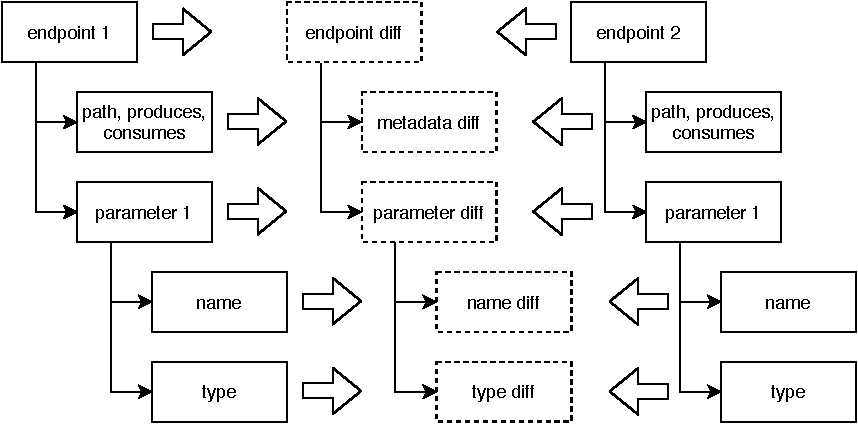
\includegraphics{diff-construction}
%	\caption{Vytvoření diffů}
%	\label{fig:diff-construction}
%\end{figure}

\section{Algoritmus porovnání}
\label{sec:cmp-alg}

Porovnávací algoritmus pracuje s metadaty popsanými v části \ref{subsec:crce-metadata}. Jedná se o stromovou strukturou, jejíž uzly tvoří instance tříd \textit{Capability}, \textit{Property} a \textit{Attribute}, kde objekty \textit{Attributes} jsou listy této struktury . Soubor metadat může obsahovat další vlastnosti komponenty, která představuje webovou službu, ta však zůstanou nedotčena, protože algoritmus pracuje pouze s daty, která byla vytvořena indexery popsanými v části \ref{sec:api-index}.

Moduly pro indexování webových služeb popsané v předchozí kapitole používají dvě různé množiny \textit{namespace} identifikátorů po pojmenování entit \textit{Capability}, \textit{Property} a \textit{Attribute}. Do budoucna je zároveň plánované rozšíření těchto modulů o funkcionalitu pro indexování datových typů a datová struktura metadat je tedy předmětem změny. Z těchto důvodů je algoritmus schopen porovnat pouze metadata vytvořená stejným indexerem a používající stejné \textit{namespace} identifikátory. Není tedy možné vzájemně porovnat například metadata REST služby získaná binární analýzou JAR s metadaty získanými čtením JSON-WSP dokumentu i když by se mohlo jednat o jednu službu.

\subsection{Popis algoritmu}

Vstupem algoritmu jsou reprezentace obou webových služeb v podobě objektů \textit{Resource}, z kterých jsou následně k porovnání vybrány kolekce endpointů, případě kolekce \textit{service} obsahující endpointy. Výstupem algoritmu je objekt \textit{Compatibility}, jež obsahuje detailní popis rozdílů mezi webovými službami ve formátu popsaném v sekci \ref{sec:diff-info}.

Před porovnáváním datových struktur je zkontrolována jejich kompatibilita. Ta je dána následujícími vlastnostmi:

\begin{itemize}
	\item typ popisu: z čeho byla metadata získána (implementace, formát popisného souboru),
	\item typ komunikace: jakým způsobem lze službu volat,
	\item \textit{identity capability}: obsahuje informace o identitě komponenty v CRCE.
\end{itemize}

Pokud kontrola proběhne úspěšně, je spuštěn samotný algoritmus jehož průběh je naznačen na vývojovém diagramu \ref{fig:apicomp-flow}. Vstupní data na obrázku označená jako \textit{endpoints1} a \textit{endpoints2} označují množiny endpointů první a druhé webové služby. 

Tento postup analogicky platí i pro porovnání \textit{service} v případě SOAP webových služeb s tím rozdílem, že krok 'Porovnej endpointy e1,e2 a výsledek ulož do res' by obsahoval porovnání endpointů definovaných v rámci jedné \textit{service}, která je v CRCE reprezentována jako kolekce endpointů. V případě porovnávání \textit{services} by množiny vstupních dat byly označené jako \textit{services1} a \textit{services2}.

\begin{figure}[h]
	\centering
	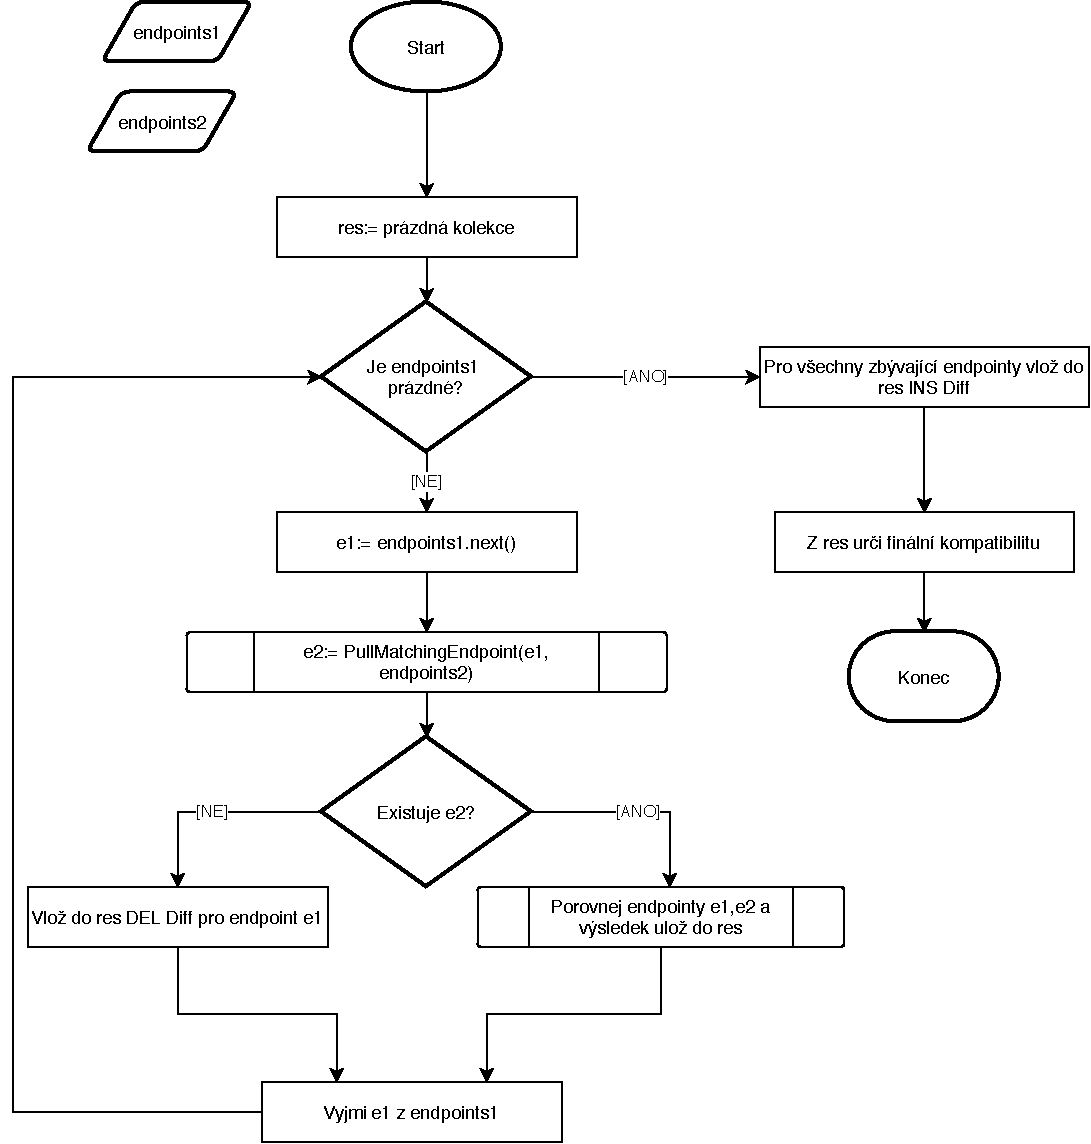
\includegraphics[width=\linewidth]{apicomp-flow}
	\caption{Vývojový diagram porovnávacího algoritmu}
	\label{fig:apicomp-flow}
\end{figure}

Mezivýsledky porovnání jsou ukládány v datové struktuře \textit{Diff}, která je detailně popsaná v sekci \ref{sec:diff-info}. Algoritmus postupuje po stromu metadat od kořene směrem k listům, ve kterých dojde k porovnání konkrétních hodnot a vyhodnocení rozdílů mezi nimi. Rozdíl mezi dvěma ne-koncovými uzly je vyhodnocen až po porovnání všech jejich potomků (nezávisle na pořadí). Algoritmus tedy postupuje zpět ke kořeni stromu, který na konci algoritmu obsahuje finální údaj o rozdílu obou služeb. Jednotlivé fáze porovnání jsou popsány v následujících odstavcích.

\subsubsection{Výběr entit vhodných k porovnání}
\label{sec:pick-matching-entities}

Tento odstavec se týká endpointů a \textit{service}, protože tyto nejsou na pořadí závislé (na rozdíl např. od parametrů operace) a jejich pořadí v metadatech nelze ani předpokládat. Proto je nutné před samotným porovnáním nejprve vybrat dvojici entit k tomu vhodnou. V diagramu \ref{fig:apicomp-flow} je zde popsaný výběr reprezentován krokem 'PullMatchingEndpoint()'. 

Endpoint \textit{e1} (\textit{service} \textit{s1})  z první webové služby je vybrán sekvenčně, jak je naznačeno na diagramu \ref{fig:apicomp-flow}. Druhý endpoint \textit{e2} (\textit{s2}) je pak vybrán na základě určité shody s metadaty endpointu \textit{e1}, respektive \textit{service s2}. V přípdě endpointů se konkrétně jedná o počet povinných parametrů, jméno a URL na které je daný endpoint dostupný. URL nemusí být shodné úplně. Pokud tak nastane, je nastavena vlajka MOV, která je detailně popsána v sekci \ref{subsec:mov}.

O porovnatelnosti a rozdílu dvou \textit{services} je rozhodnuto na základě úplné shody jejich jmen a typu (současně je používán pouze typ "\verb|rpc/messaging|").

\subsubsection{Porovnání dvou endpointů}
Po výběru vhodné dvojice endpointů dojde k jejich porovnání. Postupně se porovnají (pokud jsou pro daný typ webové služby definovány) parametry, response a těla request. Způsob porovnání parametrů a response je rozveden v následujících odstavcích. Metadata těla request jsou dostupná pouze v případě REST služeb indexovaných na základě implementace a detail jejich porovnání je znázorněn v tabulce \ref{tab:req-body-cmp}. U atributu \textit{isOptional} může dojít ke změně \textit{GEN} pokud se povinný atribut stane nepovinným. V opačném případě se jedná o změnu \textit{SPE}.

\begin{table}[h]
	\centering
	\begin{tabular}{|l|c|}
		\hline
		Název atributu  & Možné výsledky \\
		\hline
		\hline
		\textit{isArray} & \textit{NON}, \textit{UNK} \\
		\hline
		\textit{isOptional} & \textit{NON}, \textit{GEN}, \textit{SPE} \\
		\hline
		\textit{dataType} & \textit{NON}, \textit{GEN}, \textit{SPE}, \textit{UNK} \\
		\hline
	\end{tabular}
	\caption{Porovnání atributů těl requestů endpointů}
	\label{tab:req-body-cmp}
\end{table}

\subsubsection{Porovnání response dvou endpointů}

Element response je definovaný ve všech případech kromě služeb popsaných WADL. V případě REST služeb indexovaných na základě implementace jsou navíc definovány i parametry response a může také existovat více elementů response pro jeden endpoint. Ty jsou navzájem odlišeny atributem \textit{id}, jehož hodnotu vytváří indexer. Detail porovnání response (včetně parametrů) REST služeb je uveden v tabulce \ref{tab:resp-rest-cmp}, tabulka \ref{tab:resp-ws-cmp} pak obsahuje detail porovnání response ostatních služeb.

\begin{table}[h]
	\centering
	\begin{tabular}{|l|c|}
		\hline
		Název atributu & Možné výsledky \\
		\hline
		\hline
		\textit{isArray} & \textit{NON}, \textit{UNK} \\
		\hline
		\textit{dataType} &  \textit{NON}, \textit{GEN}, \textit{SPE}, \textit{UNK} \\
		\hline
		\textit{status} &  \textit{NON}, \textit{UNK} \\
		\hline
		\textit{parameterName} & \textit{NON}, \textit{UNK} \\
		\hline
		\textit{parameterCategory} & \textit{NON}, \textit{UNK} \\
		\hline
		\textit{parameterIsArray} &  \textit{NON}, \textit{UNK} \\
		\hline
		\textit{parameterDataType} & \textit{NON}, \textit{GEN}, \textit{SPE}, \textit{UNK} \\
		\hline
	\end{tabular}
	\caption{Porovnání atributů response a parametrů response endpointů REST služby}
	\label{tab:resp-rest-cmp}
\end{table}

\begin{table}[h]
	\centering
	\begin{tabular}{|l|c|}
		\hline
		Název atributu & Možné výsledky \\
		\hline
		\hline
		\textit{isArray} (pouze JSON-WSP) & \textit{NON}, \textit{UNK} \\
		\hline
		\textit{dataType} & \textit{NON}, \textit{GEN}, \textit{SPE}, \textit{UNK} \\
		\hline
	\end{tabular}
	\caption{Porovnání atributů response ostatních služeb}
	\label{tab:resp-ws-cmp}
\end{table}

\subsubsection{Porovnání parametrů endpointů}

Množiny porovnávaných atributů parametrů se navzájem liší podle typu metadat služby (viz kapitola \ref{sec:api-index}). Kompletní přehled je uveden v tabulce \ref{tab:param-cmp}. Parametry endpointů vhodné k porovnání jsou vybrány na základě jejich jména (atribut \textit{name}). Po výběru dojde k porovnání zbylých atributů a rozdíl mezi parametry je vyhodnocen na základě rozdílů mezi jejich atributy.

\begin{table}[h]
	\centering
	\begin{tabular}{|l|c|c|}
		\hline
		Název atributu & Typ metadat služby & Možné výsledky \\
		\hline
		\hline
		\textit{name} & všechny & \textit{NON}, \textit{UNK} \\
		\hline 
		\textit{dataType} & všechny & \textit{NON}, \textit{GEN}, \textit{SPE}, \textit{UNK} \\
		\hline
		\textit{order} & všechny krom WADL & \textit{NON}, \textit{UNK} \\
		\hline
		\textit{isOptional} & všechny krom WSDL & \textit{NON}, \textit{GEN}, \textit{SPE}, \textit{UNK} \\
		\hline
		\textit{isArray} & REST a JSON-WSP & \textit{NON}, \textit{UNK} \\
		\hline
		\textit{category} & REST & \textit{NON}, \textit{UNK} \\
		\hline
	\end{tabular}
	\caption{Porovnání parametrů endpointů }
	\label{tab:param-cmp}
\end{table}


\subsection{Porovnání datových typů}
\label{sec:type-cmp}
V současnosti jsou největším omezením porovnávacího algoritmu datové typy. Jak již bylo zmíněno v kapitole \ref{sec:api-index}, jméno datového typu je jedinou dostupnou informací a tedy také jediným kritériem, podle kterého je lze porovnávat. To je dostatečné v případě vestavěných typů jako například třídy z balíku \verb|java.lang|, nebo typy definované v xsd. 

Nad těmito lze provádět plnohodnotné porovnání včetně kontroly generalizace (změny \textit{GEN}, \textit{SPE}). U vestavěných typů Javy je generalizace určena na základě dědičnosti a lze například určit, že datový typ s názvem \verb|java.lang.Number| je generalizací typu s názvem \verb|java.lang.Long|, protože třída \textit{Number} je rodičem třídy \textit{Long}. Obdobně je tomu i u vestavěných typů definovaných v XSD, kde je generalizace $a <: b$ definována v případě, že typ $b$ je dost velký na pojmutí typu $a$. Například typ \verb|xsd:long| dokáže reprezentovat číslo typu \verb|xsd:int| a proto platí, že \verb|xsd:int| $<:$ \verb|xsd:long|. 

Porovnání vestavěných typů je založeno na podmínce správně zaindexovaného jména datového typu. V případě analýzy byte kódu je tato podmínka splněna, nicméně u metadat získaných čtením popisných XML souborů tomu tak vždy nemusí být. Problém spočívá v  předponě datového typu, která je součástí jeho jména a porovnávací algoritmus očekává její určitou hodnotu (konkrétně \verb|xs|). Hodnota předpony je však určena definicí namespace v XML popisu a ta se může od očekávané lišit. Tato definice není indexerem ukládána a není proto možné ji během porovnání přesně určit.

Pro uživatelsky definované typy je z těchto důvodů porovnání omezeno pouze na úplnou shodu názvu včetně prefixu, protože na základě pouhého jména datového typu nejde s jistotou usoudit nic dalšího. Změny pro jednotlivé rozdíly mezi datovými typy jsou uvedeny v tabulce \ref{tab:type-cmp}.

\begin{table}[h]
	\centering
	\begin{tabular}{|l|c|}
		\hline
		Vztah typů & Výsledek \\
		\hline
		\hline
		$ A = B$ & \textit{NON} \\
		\hline
		$ A <: B$ & \textit{GEN} \\
		\hline
		$ B <: A$ & \textit{SPE} \\
		\hline
		$ A \neq B$ & \textit{UNK} \\
		\hline
	\end{tabular}
	\caption{Rozdíly mezi datovými typy A a B}
	\label{tab:type-cmp}
\end{table}


\subsection{Časová složitost algoritmu}

Algoritmus v zásadě porovnává kolekce endpointů webových služeb a jejich počet je tedy hlavní parametr, od kterého se odvíjí časová složitost. V případě SOAP webových služeb jsou operace definované v rámci \textit{service} a je tedy třeba brát v úvahu i jejich počet. Elementární operací algoritmu je výběr vhodného páru entit (\textit{service}, nebo endpoint) a jejich následné porovnání. 

Proces výběru entit k porovnání, jež byl popsán v sekci \ref{sec:pick-matching-entities}, hledá k prvku z množiny první webové služby (\textit{endpoint1}, \textit{services1}) vhodný prvek v množině druhé webové služby (\textit{endpoints2}, \textit{services2}). Z obrázku \ref{fig:apicomp-flow} je vidět, že v případě nevhodného řazení entit bude potřeba zkontrolovat \textit{n} prvků z množiny \textit{endpoints2} (\textit{services2}), než bude nalezen vhodný protějšek k porovnání. Pokud taková situace nastane pro každý prvek z množiny první webové služby, bude potřeba provést $n*n$ výběrů a následných porovnání. V případě vhodného řazení bude naopak potřeba provést pouze $n$ výběrů, protože vhodné protějšky budou v obou množinách na stejném místě a k jejich nalezení bude vždy potřeba pouze jedno porovnání. Časová náročnost algoritmu pro jednotlivé typy služeb je shrnuta v tabulce \ref{tab:alg-complexity}.

\begin{table}[h]
	\centering
	\begin{tabular}{|l|c|}
		\hline
		Typ služby & Složitost \\
		\hline
		\hline
		REST, WADL, JSON-WSP & $\Omega(n)$, $O(n^2)$ kde $n$ je počet endpointů \\
		\hline
		WSDL & \makecell{$\Omega(mn)$, $O((mn)^2)$ kde $m$ je počet \textit{service}\\ a $n$ je počet endpointů} \\
		\hline
	\end{tabular}
	\caption{Složitost algoritmu}
	\label{tab:alg-complexity}
\end{table}
	
\section{Migrace webových služeb}	
\label{subsec:mov}
V popisu porovnání metadat endpointů bylo zmíněno použití URL endpointu jako identifikátoru. Tento přístup naráží na problém v případě, že poskytovatel ponechá nezměněnou implementaci a webovou službu přesune, nebo provede změny v cestě k danému endpointu. Na obrázku \ref{fig:mov-example} je uveden příklad dvou shodných endpointů, jež se liší pouze v URL. Aplikujeme-li výše popsaný algoritmus na tato data, skončí negativním výsledkem i přes to, že endpointy mají totožné rozhraní a klient by k nim mohl bez obtíží přistoupit. 

\begin{figure}[h]
	\centering
	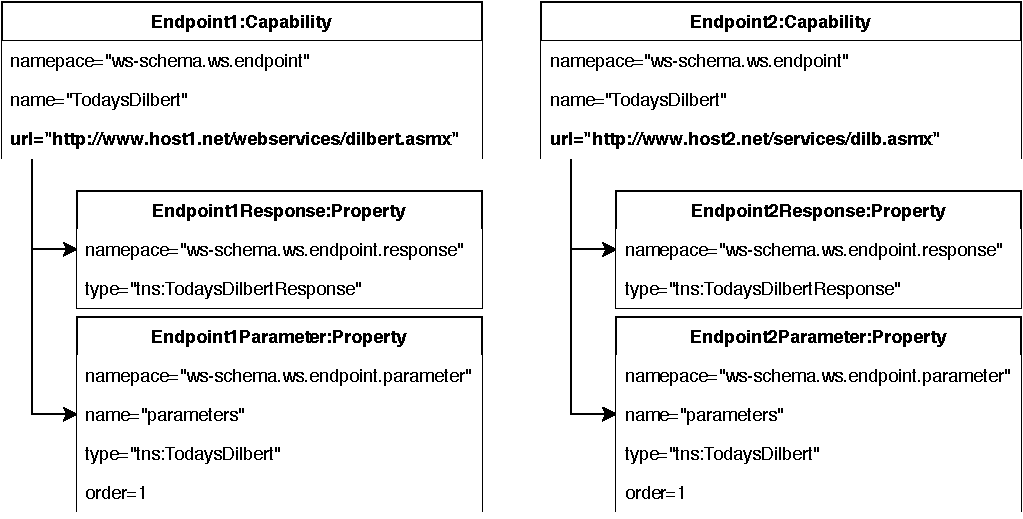
\includegraphics[width=\linewidth]{same-end-diff-url}
	\caption{Příklad shodných endpointů s rozdílnou URL}
	\label{fig:mov-example}
\end{figure}

Podobným příkladem je i verze API v cestě k endpointu. Klient může mít požadavek na zjištění kompatibility API dvou různých verzí, ale algoritmus vrátí rozdíl \textit{MUT}, protože endpointy z prvního API vyhodnotí jako chybějící v API druhém a naopak, právě kvůli rozdílným cestám. Tím vznikne kombinace rozdílů \textit{DEL} a \textit{INS}, která vede na \textit{MUT}. Takové chování není žádané a je potřeba těmto problémům předcházet, proto je nutné případné změny v URL detekovat a brát je při porovnávání v potaz.

Jako řešení popsaného problému byl zaveden příznak "MOV", který je ortogonální k úrovni změny (\textit{Difference}) popsané v předchozích sekcích a je součástí objektu \textit{Diff}. Díky ortogonalitě je možné stále určit méně nebezpečné rozdíly jako generalizaci v příznaku parametru (SPE) a zároveň předat klientovi informaci o změně v URL. 

Příznak MOV má smysl brát v úvahu jen u případů porovnání jejichž úroveň změny je v podmnožině ${NON, GEN, SPE}$, která je v rámci této sekce označována jako bezpečná. Všechny ostatní úrovně představují v kontextu migrace příliš velkou změnu. Je tedy  například nesmyslné nastavit příznak MOV u rozdílu dvou endpointů s úrovní změny \textit{DEL}, protože samotná úroveň změny říká, že endpoint nebyl v druhé webové službě nalezen a proto nelze ani určit zda byl přemístěn.  

\subsection{Detekce změn v URL}

Součástí URL endpointu je také jeho název, změny v URL se tedy dají detekovat na třech místech. Prvním z nich je doména (včetně protokolu), druhým je cesta k endpointu a třetím jeho jméno. URL všech endpointů obou webových služeb jsou podle těchto částí rozděleny, čímž vznikne 6 množin (2 pro každou část URL). Pokud platí, že $url_{i,1} \subseteq url_{i,2}$ kde $url_{i,j}$ je $i$-tá část url $j$-té webové služby, je daná část URL považována za nezměněnou. Příklad rozdělení URL dvou webových služeb vycházející z obrázku \ref{fig:mov-example} je uveden v tabulce \ref{tab:url-diff-example}. V tomto příkladu by byla detekována změna v částech URL "Doména" a "Cesta".

\begin{table}[h]
	\begin{tabular}{|l|c|c|}
		\hline
		$url_{i,j}$ & Služba 1 (j=1) & Služba 2 (j=2) \\
		\hline
		\hline
		Doména (i=1) & $\{http://host1.net\}$ & $\{http://host2.net\}$ \\
		\hline
		Cesta (i=2) & $\{webservices/dilbert.asmx\}$ &  $\{services/dilb.asmx\}$ \\
		\hline
		Operace (i=3) & $\{TodaysDilbert\}$ & $\{TodaysDilbert\}$ \\
		\hline
	\end{tabular}
	\caption{Příklad rozdělění URL na části podle obrázku \ref{fig:mov-example}}
	\label{tab:url-diff-example}
\end{table}
  
Výsledek detekce změn v URL nese tři příznaky, kde každý z nich určuje, zda byla v dané části URL detekována změna. Vzhledem k tomu, že algoritmus detekce pracuje pouze s URL a jmény endpointů, může dojde k pozitivnímu výsledku i v případě, že jsou porovnávány dvě odlišné webové služby. Aby se redukoval počet false-positives, je potřeba určit, které kombinace příznaků změny mohou vést na MOV a které představují příliš velké odchýlení. Tyto kombinace jsou uvedeny v tabulce \ref{tab:mov-explanation}, kde proměnné \textit{h}, \textit{p}, \textit{n} označují změnu v doméně, cestě a jménu endpointu. Hodnota \textit{true} značí změnu.

\begin{table}[h]
	\begin{tabular}{|l|c|c|}
		\hline
		Kombinace & MOV & Zdůvodnění \\
		\hline
		\hline
		$!h \land !p \land !n$ & ne & Nebyla detekována žádná změna. \\
		\hline
		$h \land !p \land !n$ & ano & \makecell{Změna v doméně, může se \\jednat o migraci webové služby.} \\
		\hline
		$!h \land p \land !n$ & ano & \makecell{Změna v cestě k endpointům, může se \\ jednat o restrukturalizaci služby.} \\
		\hline
		$h \land p \land !n$ & ano & Může se jednat o kombinaci obou předchozích. \\
		\hline
		všechny ostatní & ne & Změna je příliš velká. \\
		\hline
	\end{tabular}
	\caption{Kombinace změn vedoucích na MOV}
	\label{tab:mov-explanation}
\end{table}

Z tabulky je vidět, že změna ve jménech endpointů vždy vede na záporný výsledek. Jedním z důvodů je fakt, že změna ve jméně operace je mutací webové služby a jedná se tedy o nekompatibilní změnu, jejíž řešení bylo popsáno v předchozích sekcích. Dalším důvodem je použití jména endpointu jako druhého kritéria pro výběr vhodného páru endpointů (prvním je URL). Bez něj by algoritmus zdegradoval na porovnání "každý s každým",  což by značně snížilo efektivitu.   

\subsection{Výběr entit k porovnání s příznakem MOV}

Protože jedním z kritérií pro výběr vhodného páru endpointů je i URL, je potřeba upravit logiku výběru tak, aby byly brány v potaz výsledky detekce popsané v předchozí sekci. Při porovnávání URL dvou endpointů je podle kombinace změn daná část URL ignorována a pracuje se pouze s nezměněnou částí u které je vyžadována striktní rovnost.

Tento způsob může vést na případy, kdy je dvojce endpointů vyhodnocena jako potencionálně vhodná k porovnání (s nastaveným příznakem MOV), nicméně porovnání skončí negativním výsledkem, například \textit{UNK}. Pouhá akceptace takového výsledku a pokračování algoritmu by mohlo zapříčinit negativní vyhodnocení kompatibility webových služeb v případech, kdy lze mezi službami nají kompatibilní dvojice endpointů.

Příklad na obrázku \ref{fig:mov-bad-example} tento problém znázorňuje. Oba endpointy mají stejný název (atribut \textit{name}) a proto by byly vybrány jako vhodné k porovnání s nastavenými MOV příznaky $h=t$, $p=t$, $o=f$. Hlubší porovnání by však skončilo výsledkem \textit{UNK}, protože se neshodují jména a datové typy jejich parametrů a algoritmus by služby správně vyhodnotil jako nekompatibilní. V druhé webové službě by se nicméně mohl nacházet kompatibilní endpoint a je zde tedy možnost získání lepšího výsledku.

\begin{figure}[h]
	\centering
	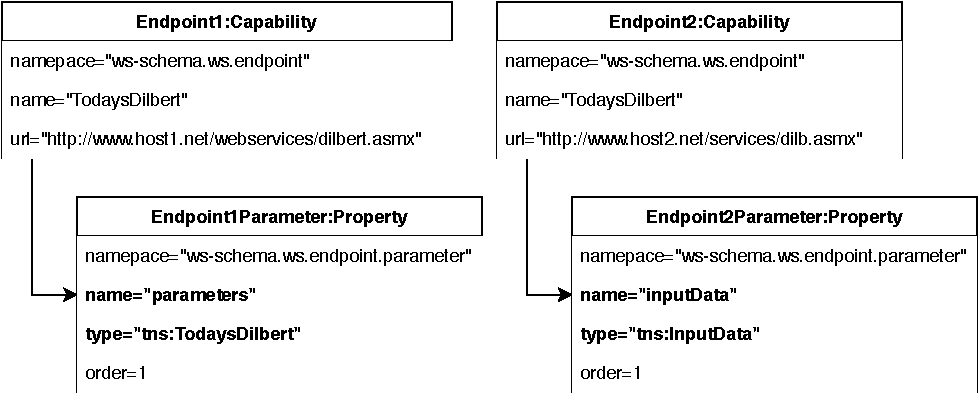
\includegraphics[width=\linewidth]{mov-example-bad}
	\caption{Příklad dvou rozdílných endpointů, pro které by byl nastaven příznak MOV}
	\label{fig:mov-bad-example}
\end{figure}

\subsubsection{Algoritmus 'pick best'}
Řešením zmíněného problému je algoritmus 'pick  best', který postupně porovnává dvojice endpointů (k tomu předem vybrané) a jako výsledek vrátí dvojici s nejlepším rozdílem. Vstupem algoritmu je tedy endpoint z první webové služby \textit{e1} a množina endpointů druhé webové služby \textit{endpoints2}. 

Algoritmus postupně vybírá elementy \textit{e2} z \textit{endpoints2} a pokud je pár $e1,e2$ vyhodnocen jako porovnatelný, dojde k detailnímu porovnání. V případě výsledku spadajícího do bezpečné množiny (${NON, GEN, SPE}$) je pár $e1,e2$ vrácen a porovnání pro endpoint \textit{e1} je ukončeno. V opačném případě je negativní výsledek uložen a z množiny \textit{endpoints2} jsou vybírány další porovnatelné endpointy dokud algoritmus nedojde ke dvojici, jejíž rozdíl spadá do bezpečné množiny, nebo dokud není \textit{endpoints2} vyčerpána. Pokud je množina \textit{endpoint2} vyprázdněna, znamená to (alespoň částečnou) nekompatibilitu obou webových služeb a je vrácen první porovnávaný pár $e1,e2$.

\subsection{Verze REST API v cestě k endpointu}	
\label{sec:api-path-version}

Jednou ze speciálních změn detekovatelných v cestě k endpointu je verze API. Jedná se o běžnou praktiku \cite{restApiVersion} a k jejímu zpracování lze použít jednodušší přístup, než byl dosud popsán. Část cesty, která obsahuje verzi lze jednoduše vypustit a porovnat URL bez verze, což případě stejného API (s odlišností verze) znamená porovnání dvou identických URL. Příznak MOV je potom nastaven pokud jsou URL s verzemi rozdílné a URL bez verzí stejné.

Algoritmus podporuje standardní verzovací formát \verb|major.minor.micro|, který je vyjádřen regulárním výrazem: \verb|/[vV][0-9]+(?:[.-][0-9]+){0,2}/|.

\section{Vyhodnocení výsledků}

Mezivýsledky porovnání jednotlivých elementů stromu metadat jsou ukládány do hierarchické struktury \textit{Diff} a vždy po vyhodnocení všech rozdílů potomků dvou uzlů, dojde na základě těchto i k vyhodnocení rozdílů uzlů samotných. Úroveň rozdílu jež určuje finální kompatibilitu webových služeb je dána úrovní kořenového \textit{Diff}, který drží celou strukturu popisující detailní rozdíly mezi službami. 

Příklad tvorby \textit{Diff} při porovnání dvou operací je znázorněn na obrázku \ref{fig:compatibility-creation}. Nejdříve dojde k vyhodnocení rozdílů listů, tedy atributů \textit{name} a \textit{type} parametrů obou operací, čímž vzniknou \textit{type diff} a \textit{name diff}. Na základě těchto se určí rozdíl mezi parametry samotnými (\textit{parameter diff}) a po porovnání metadat operací (\textit{metadata diff}) je vyhodnocen i výsledný rozdíl obou operací jež je reprezentován objektem \textit{endpoint diff}.

\begin{figure}[h]
	\centering
	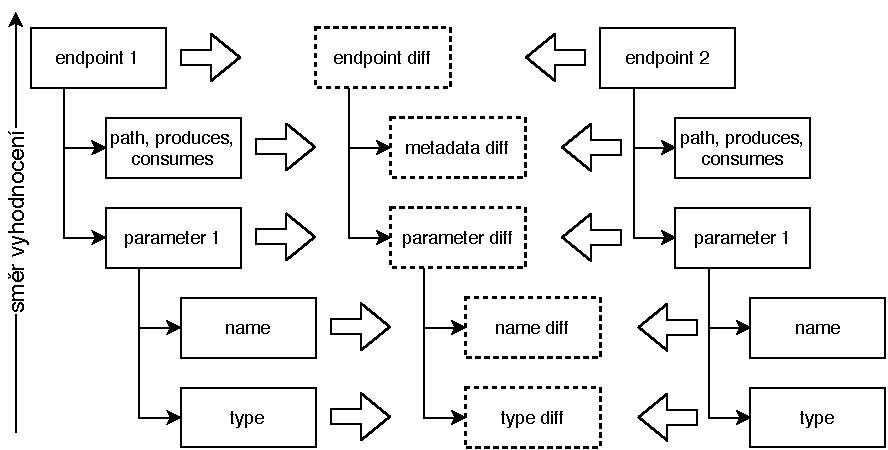
\includegraphics[height=6.5cm]{compatibility-construction}
	\caption{Tvorba rozdílů mezi dvěma endpointy}
	\label{fig:compatibility-creation}
\end{figure}

Vyhodnocení úrovně rozdílu \textit{Diff} na základě jeho potomků je řízeno prioritou. Každá z úrovní rozdílů \textit{Difference} popsaných v tabulce \ref{tab:diffs} má určitou prioritu, která reprezentuje závažnost rozdílu. Uzel od svých potomků vždy přejímá \textit{Difference} s nejvyšší prioritou, čímž je zaručeno, že se rozdíly narušující kompatibilitu projeví na finálním verdiktu.

Pokud tedy například dojde k rozdílu \textit{UNK} (maximální priorita) při porovnání dvou atributů parametru endpointu, postupným vyhodnocováním se tato \textit{Difference} dostane až ke kořenovému uzlu a výsledná kompatibilita bude mít hodnotu \textit{UNK}. Hodnoty jsou v tabulce \ref{tab:diffs} seřazeny od nejnižší priority po nejvyšší.


\subsection{Dopad na klienta}

Výše popsané úrovně \textit{Difference} mají rozdílný dopad na klienta. Ten se dá rozdělit do skupin bezpečné, potenciálně nebezpečné a nebezpečné, tak jak je tomu v tabulce \ref{tab:diff-level}. Následující odstavce popisují dopad na klienta pro jednotlivé úrovně a zdůvodňují jejich zařazení do dané skupiny.

\begin{table}[h!]
	\centering
	\begin{tabular}{|l|c|}
		\hline
		Difference & Dopad na klienta  \\
		\hline
		\hline
		None (NON) & bezpečné \\
		\hline
		Specialization (SPE) & bezpečné  \\
		\hline
		Insertion (INS) & bezpečné \\
		\hline
		Deletion (DEL) & potenciálně nebezpečné \\
		\hline
		Generalization (GEN) & potenciálně nebezpečné \\
		\hline
		Mutation (MUT) & nebezpečné \\
		\hline
		Unkown (UNK) & nebezpečné \\
		\hline
	\end{tabular}
	\caption{Dopad jednotlivých úrovní rozdílu na klienta }
	\label{tab:diff-level}
\end{table}

\subsubsection{Bezpečné rozdíly}

Pokud je rozdíl mezi službami v bezpečné skupině, může klient transparentně volat obě služby, aniž by došlo k jakékoliv chybě v rámci kontraktu. Úroveň \textit{SPE} sice označuje specializaci, nicméně změny \textit{SPE} a \textit{GEN} mohou nastat pouze v případě neshody datových typů parametrů, nebo odpovědi operace. V takovém případě je aplikován princip kontravariance \cite{abadi1995subytping} podle kterého platí, že $F'(a') <: F(a) <=> a <: a'$. \textit{SPE} tedy znamená bezpečnou změnu \textit{GEN} u parametrů, nebo odpovědi operace. 

Změna \textit{INS} nastává v případě, že druhá webová služba obsahuje operace, které nejsou v první definované. Vzhledem k tomu, že je klient nemohl volat a nemůže tak dojít k porušení kontraktu webové služby, je tato změna brána jako bezpečná.

\subsubsection{Potenciálně nebezpečné rozdíly}

Změny v této skupině mohou mít nebezpečný dopad na klienta ve smyslu volání operace webové služby s neplatným kontraktem, nicméně nejsou tak závažné jako změny nebezpečné. Posouzení reálného rizika změny provádí klient na základě vráceného objektu popisujícího kompatibilitu služeb.

Úroveň \textit{DEL} označuje element definovaný v první službě, ale chybějící v druhé. Může se jednat například o \textit{service}, nebo operaci služby. Úroveň \textit{GEN} je získána, stejně jako \textit{SPE}, na základě principu kontravariance a označuje změnu v datovém typu (parametru, odpovědi operace, ...), například z \textit{long} na \textit{int}. 

\subsubsection{Nebezpečné rozdíly}

Změny v této skupině představují buď kombinace několika méně závažných změn (\textit{MUT}), nebo neporovnatelnost obou webových služeb (\textit{UNK}). Stejně jako u předchozí skupiny, i zde může klient použít výsledky porovnání a sám rozhodnout o míře nekompatibility. Úroveň \textit{MUT} může například nastat i kombinací rozdílů endpointů, které klient nepoužívá a druhá webová služba tak pro něj může být stále kompatibilní.

Úroveň \textit{UNK} označuje buď neporovnatelnost metadat a v takovém případě nelze o kompatibilitě jednoznačně rozhodnout, nebo nerovnost metadat v případě, kde možným výsledkem je pouze 'stejné', nebo 'nestejné'.


\chapter{Implementace rozšíření}
\label{sec:impl}

Cílem mé práce bylo vytvořit rozšíření CRCE schopné automatické kontroly kompatibility indexovaných webových služeb. V předchozí kapitole byl představen algoritmus pro porovnání dvou webových služeb na základě jejich metadat a následného vyhodnocení výsledků. Tato kapitola popisuje způsob implementace algoritmu jako rozšiřujícího modulu pro systém CRCE.

První část kapitoly, v návaznosti na zmíněnou modulární architekturu CRCE, rozebírá způsob jeho rozšíření a integraci nových modulů. V druhé části je pak uveden stručný popis implementačních detailů výše zmíněného modulu, včetně procesu automatizovaného sestavení a nasazení celého CRCE.

\section{Rozšíření CRCE}

V kapitole \ref{sec:crce} byla zmíněna modulární architektura CRCE, jehož jednotlivé moduly jsou tvořeny OSGi bundly v podobě maven artefaktů. Základní funkcionalita CRCE je rozprostřena mezi několik modulů tvořící jádro. Ostatní moduly představující nadstavbou jádra jsou podřazené modulu \verb|crce-modules-reactor| a zde je umístěno i mnou vytvořené rozšíření.

\subsection{Integrace modulu}

Modul ke své správné funkčnosti vyžaduje několik dalších komponent. Tato závislost je znázorněna na obrázku \ref{fig:apicomp-crce-interaction}, porovnávací modul je zde zeleně označený. Konkrétně se jedná o moduly \textit{crce-core}, který sdružuje všechny komponenty jádra (takže není nutné definovat závislosti jednotlivě) a \textit{crce-compatibility-dao-api}, který obsahuje rozhraní pro přístup k datovému úložišti objektů \textit{Compatibility}. 

Výsledky porovnání webových služeb jsou ukládány do perzistentního úložiště a není tedy nutné znovu počítat rozdíly pro již porovnané dvojice. Ukládání těchto dat obstarává modul \textit{crce-compatibility-dao-mongodb}, jež implementuje výše  zmíněné rozhraní. V rámci mé práce jsem tyto moduly rozšířil o funkcionalitu pro získání objektu \textit{Compatibility} podle zadané dvojice \textit{Resource} a mazání existujících objektů \textit{Compatibility}.

\begin{figure}[h]
	\centering
	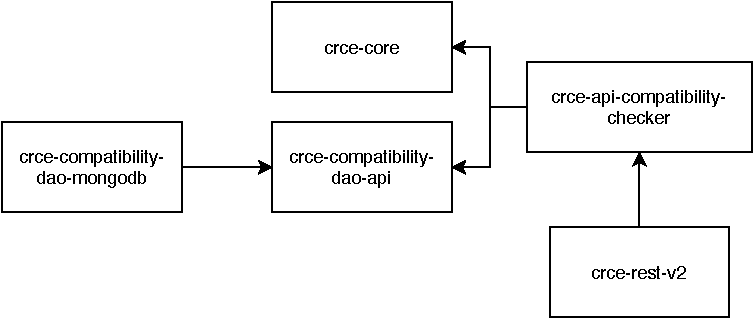
\includegraphics[width=10cm]{module-integration}
	\caption{Interakce rozšíření se zbytkem CRCE}
	\label{fig:apicomp-crce-interaction}
\end{figure}

\section{Porovnávací rozšíření}

Vnitřně je struktura modulu rozdělena na několik částí. Těmi nejdůležitějšími jsou část implementační nacházející se v balíku \verb|impl|, část pro reprezentaci výsledků v balíku \verb|result| a veřejné rozhraní porovnávací služby v \textit{ApiCompatibilityCheckerService}. Implementace tohoto rozhraní je zpřístupněná formou OSGi služby (anotace \textit{Component}), v níž jsou obsaženy všechny porovnávače jednotlivých typů webových služeb a implementace sama je schopná vybrat správný porovnávač pro zadanou dvojici \textit{Resource}.

\subsection{Struktura tříd porovnávačů}

Diagram \ref{fig:cmp-uml-class} znázorňuje strukturu tříd, jež slouží k porovnávání webových služeb. Každý porovnávač dědí od abstraktní třídy \textit{ApiCompatibilityChecker}, která obsahuje deklaraci metody určené k porovnání služeb (\textit{compareApis()}). Z důvodů zmíněných v sekci \ref{sec:cmp-alg} je algoritmus implementován ve dvou verzích (na obrázku zeleně vyznačené třídy) podle původu metadat. První verze (na obrázku \textit{RestApiCompatibilityChecker}) pracuje s metadaty získanými z implementace služby, druhá (na obrázku \textit{WebservicesCompatibilityChecker}) pak s metadaty získanými z popisu webové služby.

% - zmínit, proč třídy pro porovnávání REST API a WS nemají společného předka (krom rozhraní)
% 	- důvod: chtěl jsem nechat implementaci obou porovnávačů oddělenou pro případ, že by se změnila funkce indexerů

\begin{figure}[h]
	\centering
		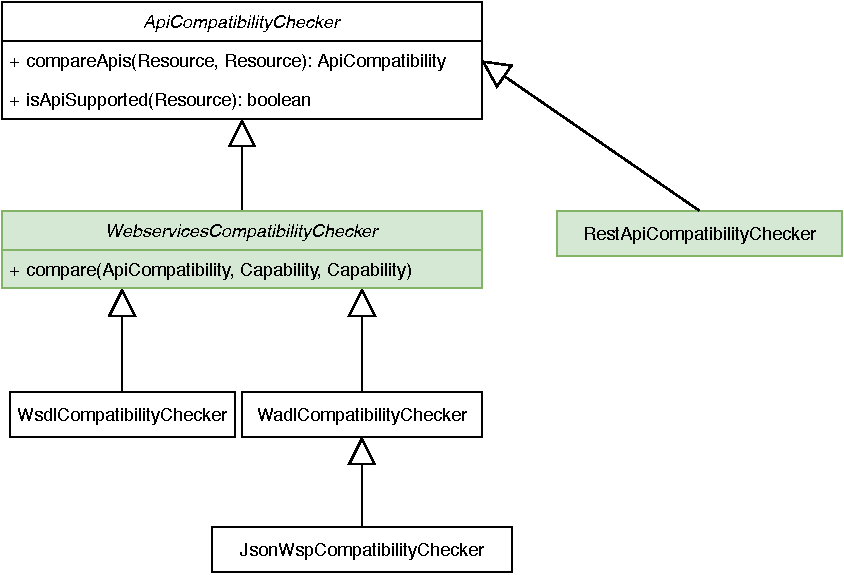
\includegraphics[width=\linewidth]{cmp-uml-class}
	\caption{Diagram tříd popisující strukturu porovnávače}
	\label{fig:cmp-uml-class}
\end{figure}

I když je struktura metadat podobná, rozhodl jsem se vytvářet co možná nejméně společné implementace, protože bych tím vytvořil silnou vazbu mezi jinak nezávislými indexery. Ta by v případě změny struktury metadat u jednoho z indexerů přinášela obtíže při následné refaktorizaci porovnávacího modulu. Jediným společným předkem je tedy obecná abstraktní třída pro porovnávač webových služeb.

Protože indexer pracující s popisem je schopen indexovat více typů služeb, je pro každý z těchto typů vytvořen zvláštní porovnávač. Na obrázku to jsou třídy dědící od \textit{WebservicesCompatibilityChecker}. Tato obsahuje porovnávací logiku a abstraktní metody pro získání konkrétních detailů jako například jmen některých atributů, identifikátorů \textit{Capability}, nebo instancí porovnávačů metadat, které jsou použité během porovnání. Daná implementace pak tyto metody překrývá čímž poskytuje data specifická danému typu služby.

\subsubsection{Porovnávání endpointů}

Jak bylo zmíněno v kapitole \ref{sec:cmp-alg}, porovnávání endpointů služeb je rozděleno na několik částí. Z důvodů čistoty kódu a principu jedné odpovědnosti je logika porovnání každé části umístěna ve zvláštní třídě a pro každé jedno porovnání je vytvořena nová instance této třídy. Obrázek \ref{fig:endpoint-cmp-uml-class} obsahuje diagram těchto tříd společně s abstraktní třídou od které dědí každý z porovnávačů. 

\begin{figure}[h]
	\centering
	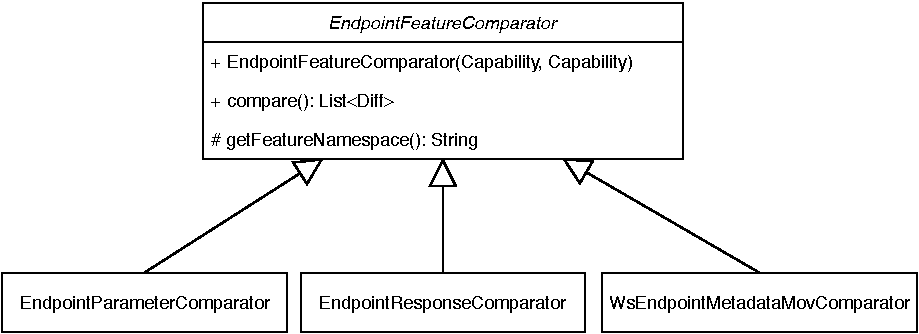
\includegraphics[width=\linewidth]{endpoint-cmp-uml-class}
	\caption{Struktura porovnávače vlastností endpointů}
	\label{fig:endpoint-cmp-uml-class}
\end{figure}

Abstraktní třída \textit{EndpointFeatureComparator} obsahuje pouze extrakci daných vlastností endpointů z objektů \textit{Capability} a abstraktní metodu \textit{compare()}, kterou volá klientský kód. Tím je dosaženo snadné rozšiřitelnosti v případě nutnosti porovnání dalších vlastností endpointu, například pokud by se rozšířila struktura metadat. 

\subsubsection{Vestavěné datové typy}

Porovnávání vestavěných datových typů je řešeno obalovací třídou, jejíž vstupním parametrem je jméno obalovaného datového typu. Tato třída obsahuje logiku která je schopná vyhodnotit, zda se doopravdy jedná o jméno vestavěného typu a také logiku porovnání dvou vestavěných typů. V současné době je toto porovnání omezeno na rovnost a generalizaci (jak bylo uvedeno v sekci \ref{sec:type-cmp}). Konkrétní obalové třídy jsou \textit{JavaTypeWrapper} pro vestavěné typy Javy a \textit{XsdDataType} pro vestavěné typy XML. 

Obalové třídy nepokrývají všechny vestavěné typy, ale pouze jejich podmnožinu. Zejména se jedná o čísla (i s plovoucí desetinnou čárkou) a řetězce.

\section{Sestavení a nasazení modulu}

Jedním z hlavních bodů oborového projektu, který předcházel této diplomové práci bylo zprovoznění automatického sestavení a nasazení CRCE do vývojového prostředí. Toho jsem využil při vývoji porovnávacího modulu zejména k rychlému nasazení nových verzí, které pak bylo možné pohodlně otestovat. Sestavením CRCE na nezávislém stroji jsem zároveň ověřil, že mnou vytvořený kód netrpí chybami typu "funguje na mém stroji".

Kód CRCE je udržován na univerzitním Gitlabu, který kromě podpory verzování nástrojem GIT umožňuje také kontinuální integraci a nasazení pomocí Gitlab Pipelines\footnote{https://docs.gitlab.com/ee/ci/pipelines/index.html}. Vstupem tohoto nástroje je deklarativní konfigurace jednotlivých kroků od překladu až po nasazení. Pipeline se automaticky spustí vždy při nahrání nového commitu do úložiště. Součástí nakonfigurované pipeline je také spuštění unit testů.

Soubor \verb|.gitlab-ci| obsahující nastavení pipeline ve formátu YAML se nachází v kořenovém adresáři projektu a obsahuje definici kroků pro sestavení a následné nasazení do testovacího prostředí. Obrázek \ref{fig:pipeline-example} znázorňuje příklad zjednodušené pipeline, její plná verze je uvedena v přiloženém archivu obsahujícím zdrojový kód CRCE. 

\begin{figure}
	\centering
	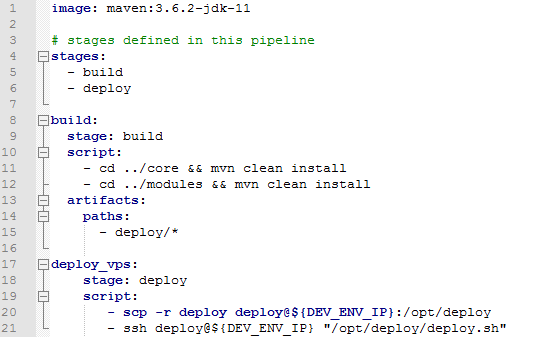
\includegraphics[width=\linewidth]{pipeline-example}
	\caption{Příklad konfigurace Gitlab pipeline}
	\label{fig:pipeline-example}
\end{figure}

\chapter{Ověření funkčnosti}
\label{sec:testing}

Rozšíření do systému CRCE, jež bylo předmětem mé práce bylo testováno jednotkovými a integračními testy. Tato kapitola se postupně ve třech částech zabývá použitím modulu a ověřením jeho správné funkčnosti. V první části je rozebráno spuštění a použití modulu od nahrání artefaktů do CRCE až po získání výsledků porovnání. Druhá část této kapitoly obsahuje popis integračních testů, včetně testovacích dat. Na konci kapitoly jsou shrnuty provedené testy a jejich výsledky.

\section{Spouštění modulu}

Na rozdíl od indexerů zmíněných v kapitole \ref{sec:api-index} není modul pro počítání kompatibility přímo napojen na žádnou z fází životního cyklu komponenty v CRCE a je potřeba jej manuálně spouštět. V současné době je rozšíření zpřístupněno skrze REST API implementovaném v modulu \textit{crce-rest-v2}. Zde je pomocí dependency injection zpřístupněná služba \textit{ApiCompatibilityCheckerService}, která na základě předaných vstupních parametrů provede porovnání a vrátí výsledek v podobě objektu \textit{Compatibility}. Ten je pak vrácen klientovi. Endpoint na němž je zpřístupněn porovnávací modul je dostupný na URI:
\begin{figure}[h]
\centering
\verb|http://69.90.132.97:8080/rest/v2/apicomp/compare|
\end{figure}

Parametry volání jsou uvedeny v tabulce \ref{tab:rest-cmp-params}. Nepovinný parametr \textit{force}, jehož výchozí hodnota je \textit{false} byl přidán z důvodů nutnosti přepočítání výsledků v případě změny implementace. Pokud tedy dojde například k opravě chyby díky které jsou v databázi uložena špatná data, není nutné je ručně mazat, ale stačí porovnání spustit znovu s nastaveným příznakem \textit{force}. Příklady volání API a následně vrácených dat jsou v následující podkapitole.

\begin{table}[h]
	\centering
	\begin{tabular} {|l|c|c|}
		\hline
		Název & Popis & Povinný \\
		\hline
		\hline
		id1 & ID 1. \textit{Resource} k porovnání & Ano \\
		\hline
		id2 & ID 2. \textit{Resource} k porovnání & Ano \\
		\hline
		force & Ignorovat existující \textit{Comaptibility} & Ne \\
		\hline		
	\end{tabular}
	\caption{Parametry volání endpointu pro porovnání služeb}
	\label{tab:rest-cmp-params}
\end{table}

\section{Použití modulu}
\label{sec:module-how-to}

Aby bylo možné modul použít, je nejprve potřeba nahrát testovací data. Tato sekce popisuje proces nahrání artefaktu obsahujícího implementaci webové služby, do CRCE a jeho následného porovnání se sebou samým. Uživatelské rozhraní testovací instance systému CRCE je dostupné na adrese:

\begin{figure}[h]
	\centering
	\verb|http://69.90.132.97:8080/crce-webui/|
\end{figure}

\paragraph{Nahrání artefaktu do CRCE}

Uživatelské rozhraní pro nahrávání artefaktů je zpřístupněno pod položkou  \textit{File/url} menu \textit{Upload}. Zde je možné tlačítkem \textit{Browse files} vybrat artefakt (v tomto případě \textit{jersey-test-1.war})  a potvrdit nahrání, po jehož dokončení se v pravém horním rohu zobrazí zpráva oznamující úspěch, viz obrázek \ref{fig:crce-art-upload}.

\begin{figure}[h]
	\centering
	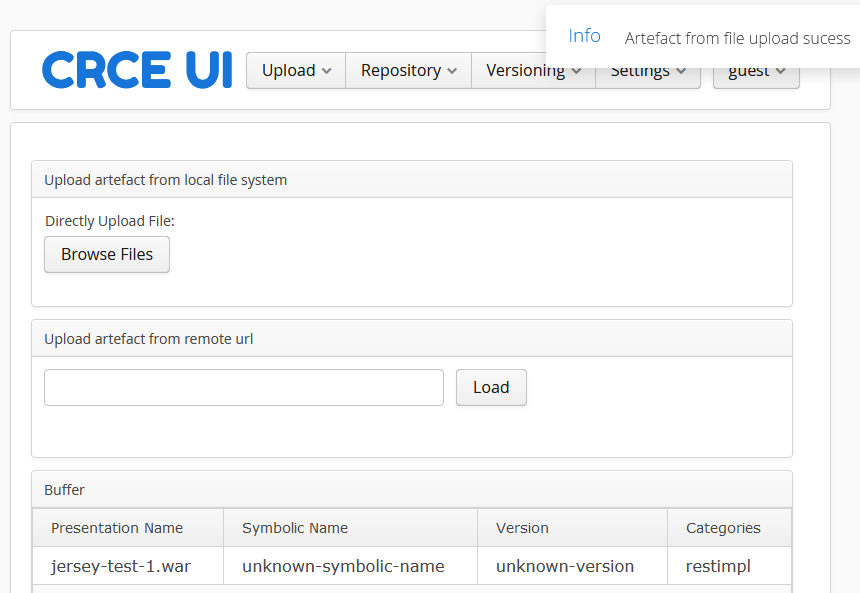
\includegraphics[width=\linewidth]{crce-art-upload.png}
	\caption{Nahrání artefaktu s implementací webové služby do CRCE}
	\label{fig:crce-art-upload}
\end{figure}

\paragraph{Nahrání artefaktu do Store}
V tuto chvíli se nahraná komponenta nachází ve fázi \textit{Buffer}. Došlo tedy k získání metadat a indexaci artefaktu, nicméně pro porovnání je nutné provést operaci \textit{commit} a tím komponentu posunout do fáze \textit{Store}. To lze udělat tlačítkem \textit{Push to Store} v záložce \textit{Plugins} pod menu \textit{Repository}, jak je znázorněno na obrázku \ref{fig:crce-art-push-to-store}. Tato záložka mimo jiné obsahuje přehled všech komponent nacházejících se ve fázi \textit{Buffer} svého životního cyklu.

\begin{figure}[h]
	\centering
	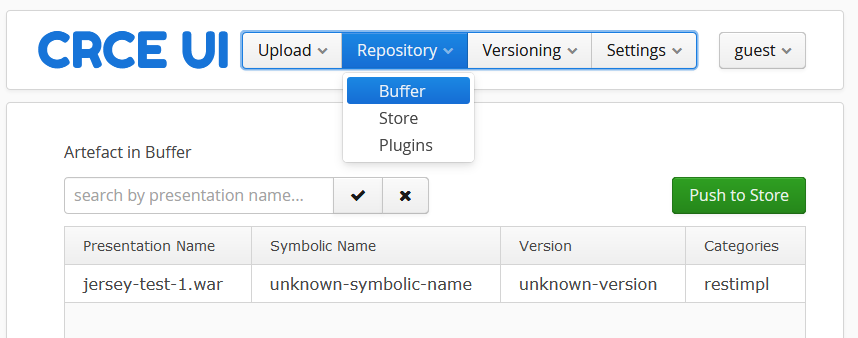
\includegraphics[width=\linewidth]{crce-art-push-to-store.png}
	\caption{Nahrání artefaktu s implementací z Buffer do Store}
	\label{fig:crce-art-push-to-store}
\end{figure}

\paragraph{Získání ID artefaktu}
K porovnání webových služeb je nutné znát ID \textit{Resource}, jež reprezentují nahrané artefakty. Označením daného artefaktu v tabulce se zobrazí menu s akcemi \textit{Detail} a \textit{Remove} pro daný artefakt. Kliknutím na tlačítko \textit{Detail} je zobrazena stránka s metadaty artefaktu, včetně seznamů \textit{Capability} a \textit{Requirement}. Detail artefaktu nahraného v předchozím kroku je na obrázku \ref{fig:crce-art-detail}.

\begin{figure}[h]
	\centering
	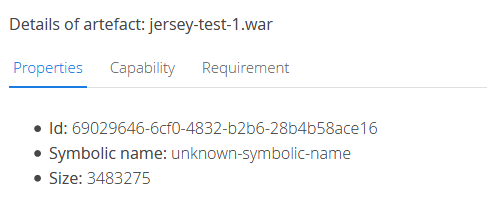
\includegraphics[width=10cm]{crce-art-detail.png}
	\caption{Detail nahraného artefaktu}
	\label{fig:crce-art-detail}
\end{figure}

\paragraph{Volání porovnávací služby}
Identifikátor získaný v předchozím kroku lze použít k volání REST služby pro porovnávání. K tomu jsem pro jednoduchost použil nástroj Postman. Protože se tento příklad zabývá pouze jedním artefaktem, jsou parametry \textit{id1} a \textit{id2} totožné. Příklad volání služby s danými identifikátory je na obrázku \ref{fig:apicomp-call}.

\begin{figure}[h]
	\centering
	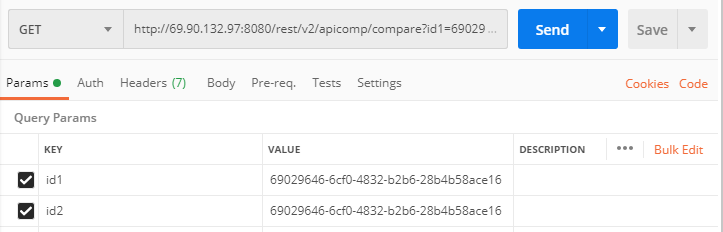
\includegraphics[width=\linewidth]{apicomp-call.png}
	\caption{Volání porovnávací služby}
	\label{fig:apicomp-call}
\end{figure}

\paragraph{Výsledky porovnání}
Výsledek vrácený porovnávací službou je uveden na obrázku \ref{fig:apicomp-res}. Pro jednoduchost jsou některé části výsledného JSON dokumentu vypuštěny. Ve výsledku je obsažena finální úroveň rozdílu (\textit{diffValue}), příznaky nastavené během porovnání (\textit{additionalInfo}) a také strukturu \textit{diffDetails} tvořenou stromem objektů \textit{Diff} detailně popisující rozdíly mezi službami.

\begin{figure}[h]
	\centering
	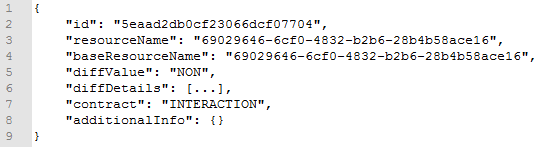
\includegraphics[width=\linewidth]{apicomp-res.png}
	\caption{Volání porovnávací služby}
	\label{fig:apicomp-res}
\end{figure}

Pokud by během porovnání došlo k nastavení příznaku MOV, byl by tento vrácený v \textit{additionalInfo}. Protože byl artefakt porovnán sám se sebou, je výsledný rozdíl \textit{NON}.

\section{Testování}

Funkčnost modulu byla ověřena pomocí několika testovacích scénářů, jejichž účelem je otestování změn v rozhraní webových služeb vedoucích na kompatibilní i nekompatibilní rozdíly. Každý ze scénářů je zaměřen na jeden typ indexované služby a všechny s CRCE komunikují skrze REST API, tak jak bylo popsáno v předchozí sekci. Vstupní data pro tyto scénáře byla získána z kombinace reálných i synteticky vytvořených služeb. Premisou pro úspěch testů je správná funkčnost indexovacích modulů popsaných v části \ref{sec:api-index} kapitoly \ref{sec:crce}. Ta byla ověřena analýzou implementace společně s manuálním testováním, během kterého byla objevena a opravena chyba ve zpracování WSDL dokumentu, rovněž popsaná v sekci \ref{sec:api-index}.

Princip každého z testovacích scénářů spočívá ve vytvoření několika verzí jedné služby (případně jejího popisu) a následném vzájemném porovnání. Tím lze otestovat jak vybrané změny tak i závislost výsledku na pořadí porovnávaných služeb. Jednotlivé scénáře včetně výsledků jsou detailně popsány v následujících sekcích.

K testování jsem použil nástroj Postman, konkrétně jeho Collection Runner, který umožňuje vybrat šablonu volání REST API a soubor testovacích dat ve formátu CSV. jehož každá řádka představuje jeden test v podobě identifikátorů porovnávané dvojice služeb a očekávaného výsledku. Nástroj Collection Runner tento soubor čte po řádcích a data z každé řádky aplikuje na zmíněnou šablonu. Tím lze snadno zautomatizovat testování volání webové služby s mnoha kombinacemi vstupních dat. Příklad těchto datového souboru je uveden na obrázku \ref{fig:test-data-csv}. 

\begin{figure}[h]
	\centering
	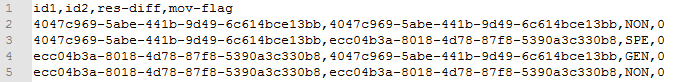
\includegraphics[width=\linewidth]{test-data-csv.png}
	\caption{Příklad testovacích dat pro nástroj Postman}
	\label{fig:test-data-csv}
\end{figure}

Test, zda výsledek volání odpovídá datům uvedeným v CSV souboru provádí skript napsaný v jazyce JavaScript, jež je součástí zmíněné šablony volání (k dispozici na přiloženém CD). Příklad výsledků testů vrácených nástrojem Collection Runner je zobrazen na obrázku \ref{fig:test-results}.

\begin{figure}[h]
	\centering
	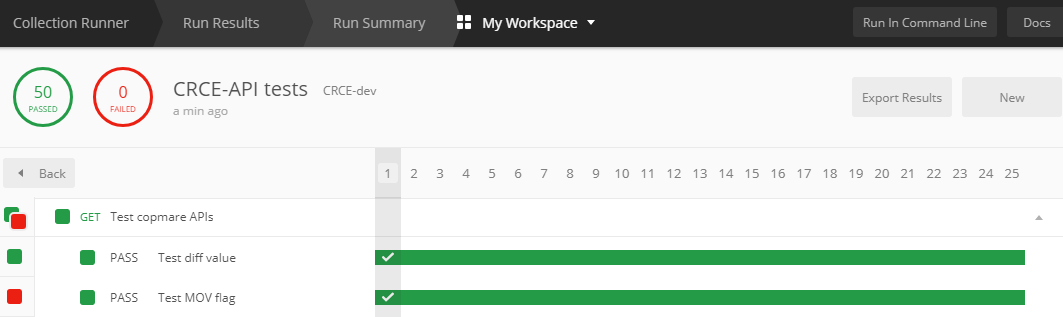
\includegraphics[width=\linewidth]{test-results.png}
	\caption{Výsledek testování nástrojem Postman}
	\label{fig:test-results}
\end{figure}


\subsection{REST služba založená na Jersey}

V tomto scénáři jsou testovány dvě verze REST služby implementované frameworkem Jersey\footnote{https://eclipse-ee4j.github.io/jersey/}. Metadata služby byla získána nahráním její implementace do CRCE způsobem popsaným v sekci \ref{sec:module-how-to}. Popis rozhraní obou verzí služby se nachází na přiloženém CD.  

Rozdíl mezi jednotlivými verzemi je pouze v datovém typu parametru \textit{longParam} endpointu \textit{myresource/special/pet/}. V první verzi je tento parametr typován na \textit{java.lang.Number}, v druhé pak na \textit{java.lang.Long}.

Účelem tohoto testovacího scénáře je kromě ověření funkčnosti modulu pro indexaci REST služeb z bytecode také ověření správné aplikace principu kontravariance v případě změn datových typů parametrů endpointů. Změna datového typu z \textit{Long} na \textit{Number} je změnou \textit{GEN}. Po použití kontravariance by změna na úrovni endpointu měla být \textit{SPE} a protože je to jediný rozdíl mezi službami, měla by tato změna označovat také celkový rozdíl.

Výsledky vrácené voláním porovnávací služby jsou zobrazeny v tabulce \ref{tab:jersey-cmp-res}. Výsledky odpovídají očekávání a princip kontravariance v případě změn \textit{GEN} a \textit{SPE} u datového typu parametru endpointu služby je tedy aplikován správně.

\begin{table}[h]
	\centering
	\begin{tabular}{|l||c|c|}
		\hline
		& v1 & v2 \\
		\hline
		\hline
		v1 & \textit{NON} & \textit{SPEC} \\
		\hline
		v2 & \textit{GEN} & \textit{NON} \\
		\hline
	\end{tabular}
	\caption{Výsledky porovnání metadat získaných z implementace}
	\label{tab:jersey-cmp-res}
\end{table}
	
\subsection{Služba popsaná JSON-WSP}

Testovací scénář je zaměřen na služby popsané formátem JSON-WSP. Vstupní metadata byla získána indexováním čtyř verzí popisu uměle vytvořeného rozhraní založeného na příkladu převzatém z Wikipedie\footnote{https://en.wikipedia.org/wiki/JSON-WSP}. Odlišnosti mezi jednotlivými verzemi, označenými \textit{v1} až \textit{v4}, jsou rozepsány v tabulce \ref{tab:json-wsp-diffs}. Všechny verze popisů rozhraní služby jsou umístěny na přiloženém CD.

\begin{table}[h]
	\centering
	\begin{tabular}{|l|c|}
		\hline
		Verze služby & Popis změny \\
		\hline
		\hline
		v1 & Základní verze \\
		\hline
		v2 & Modifikace datového typu \textit{User} \\
		\hline
		v3 & Přidána operace \textit{deleteUser} \\
		\hline
		v4 & Operace \textit{listGroups} změněna na \textit{getUserInGroup} \\
		\hline
	\end{tabular}
	\caption{Přehled změn ve verzích služby}
	\label{tab:json-wsp-diffs}
\end{table}

Účelem tohoto scénáře je ověřit porovnávání vlastních datových typů a mutací mezi endpointy. Verze služby \textit{v2} mění definici typu \textit{User}, ale ne jeho název. Vzhledem k faktu, že definice typů nejsou indexovány, mělo by porovnání skončit výsledkem \textit{NON}, protože názvy typů se shodují. Verze \textit{v3} a \textit{v4} přidávají endpointy, čímž mutují rozhraní služby. Očekávané výsledky pro tyto verze jsou \textit{INS} pro \textit{v3} (přidaný endpoint) a \textit{MUT} pro \textit{v4} (změna názvu operace).

Tabulka \ref{tab:jsonwsp-cmp-res} obsahuje výsledky vrácené porovnávací službou, které odpovídají předpokladům uvedeným v předchozím odstavci.

\begin{table}[h]
	\centering
	\begin{tabular}{|l||c|c|c|c|}
		\hline
		& v1 & v2 & v3 & v4 \\
		\hline
		\hline
		v1 & \textit{NON} & \textit{NON} & \textit{INS} & \textit{MUT} \\
		\hline
		v2 & \textit{NON} & \textit{NON} & \textit{INS} & \textit{MUT} \\
		\hline
		v3 & \textit{DEL} & \textit{DEL} & \textit{NON} & \textit{MUT} \\
		\hline
		v4 & \textit{MUT} & \textit{MUT} & \textit{MUT} & \textit{NON} \\
		\hline
	\end{tabular}
	\caption{Výsledky porovnání metadat získaných z JSON-WSP popisu}
	\label{tab:jsonwsp-cmp-res}
\end{table}


\subsection{Služba FuelEconomy}

Tento scénář je zaměřen na porovnání REST služeb, jejichž rozhraní je popsáno WADL dokumentem. Metadata, jež jsou vstupem tohoto testu, byla získána indexováním popisu rozhraní služby Fuel Economy\footnote{https://www.fueleconomy.gov/ws/rest/application.wadl} a z něj vycházejících tří modifikovaných verzí. Popis změn jednotlivých verzí oproti verzi \textit{v1} je uveden v tabulce \ref{tab:wadl-diffs}. Všechny verze WADL dokumentu jsou na přiloženém CD.

\begin{table}[h]
	\centering
	\begin{tabular}{|l|c|}
		\hline
		Verze služby & Popis změny \\
		\hline
		\hline
		v1 & Základní verze \\
		\hline
		v2 & Odebrán resource \textit{labelvehicle} \\
		\hline
		v3 & \makecell{Odebrán resource \textit{labelvehicle}, \\ přidán resource \textit{somethingDifferent}} \\
		\hline
		v4 & \makecell{Změna URL a změna cesty z \textit{/fuelprices} na \textit{fuel-prices}}  \\
		\hline
	\end{tabular}
	\caption{Přehled změn ve verzích služby}
	\label{tab:wadl-diffs}
\end{table}

Scénář je zaměřen na mutaci operací a změny v URL na kterých jsou dostupné. Verze \textit{v2} a \textit{v3} testují mutaci, konkrétně přidávání a odebírání operací. Očekávané výsledky jsou \textit{DEL} v případě \textit{v2} a \textit{MUT} V případě \textit{v3}. Verze služby \textit{v4}, kde jedinou změnou je URL a cesta k endpointu \textit{fuelprices}, testuje správné nastavení příznaku \textit{MOV} a očekávaný rozdíl je \textit{NON}.

\begin{table}[h]
	\centering
	\begin{tabular}{|l||c|c|c|c|}
		\hline
		& v1 & v2 & v3 & v4 \\
		\hline
		\hline
		v1 & \textit{NON} & \textit{DEL} & \textit{MUT} & \textit{NON},\textit{MOV} \\
		\hline
		v2 & \textit{INS} & \textit{NON} & \textit{INS} & \textit{INS} \\
		\hline
		v3 & \textit{MUT} & \textit{DEL} & \textit{NON} & \textit{MUT} \\
		\hline
		v4 & \textit{NON},\textit{MOV} & \textit{DEL} & \textit{MUT} & \textit{NON} \\
		\hline
	\end{tabular}
	\caption{Výsledky porovnání metadat získaných z WADL popisu}
	\label{tab:wadl-cmp-res}
\end{table} 

V tabulce \ref{tab:wadl-cmp-res} jsou obsaženy výsledky vzájemného porovnání jednotlivých verzí služby. Pro přehlednost je v tabulce uveden příznak MOV pouze v případě, že byl vrácen. Pokud nastaven nebyl, je v tabulce uveden pouze rozdíl služeb. 

\subsection{Služba STAG-Číselníky}

Testovací scénář je zaměřen na SOAP služby popsané dokumentem ve formátu WSDL. Vstupní metadata byla získána indexováním popisu rozhraní služby STAG-Číselníky\footnote{https://stag-ws.zcu.cz/ws/services/soap/ciselniky?wsdl} a z něj vycházejících čtyř modifikovaných verzí. Celkem je tedy porovnáno pět verzí, jejichž rozdíly jsou popsané v tabulce \ref{tab:wsdl-diffs}. Všechny verze WSDL dokumentu popisující rozhraní této služby se nachází na přiloženém CD.

\begin{table}[h]
	\centering
	\begin{tabular}{|l|c|}
		\hline
		Verze služby & Popis změny \\
		\hline
		\hline
		v1 & Základní verze s přidanou operací \textit{testOperation} \\
		\hline
		v2 & Změna hostname v url operací \\
		\hline
		v3 & Změna typu \textit{insertPracoviste} \\
		\hline
		v4 & \makecell{Změna názvu \textit{service} z \textit{CiselnikyServiceImplService} na \\ \textit{CiselnikyServiceImplServiceUpdate}}  \\
		\hline
		v5 & \makecell{Změna typu parametru operace \textit{testOperation} \\
		z \textit{xs:int} na \textit{xs:long}} \\ \hline
	\end{tabular}
	\caption{Přehled změn ve verzích služby}
	\label{tab:wsdl-diffs}
\end{table}

Základní verze \textit{v1} byla rozšířena o operaci \textit{testOperation}, která má nastavený parametr typovaný na \textit{xs:int}. Porovnání verze \textit{v1} s verzemi \textit{v2} a \textit{v5} je využito k testování principu kontravariance společně se změnami v URL. Verze \textit{v3} mění definici typu \textit{insertPracoviste}. Tato změna by neměla porovnání nijak ovlivnit, protože detaily vlastních datových typů nejsou indexovány. Verze \textit{v4} mění název \textit{service}, což by mělo být vyhodnoceno jako mutace.

\begin{table}[h]
	\centering
	\begin{tabular}{|l||c|c|c|c|c|}
		\hline
		& v1 & v2 & v3 & v4 & v5 \\
		\hline
		\hline
		v1 & \textit{NON} & \textit{NON},\textit{MOV} & \textit{NON} & \textit{MUT} & \textit{SPE} \\
		\hline
		v2 & \textit{NON},\textit{MOV} & \textit{NON} & \textit{NON},\textit{MOV} & \textit{MUT} & \textit{SPE},\textit{MOV} \\
		\hline
		v3 & \textit{NON} & \textit{NON},\textit{MOV} & \textit{NON} & \textit{MUT} & \textit{SPE} \\
		\hline
		v4 & \textit{MUT} & \textit{MUT} & \textit{MUT} & \textit{NON} & \textit{MUT} \\
		\hline
		v5 & \textit{GEN} & \textit{GEN},\textit{MOV} & \textit{GEN} & \textit{MUT} & \textit{NON} \\
		\hline
	\end{tabular}
	\caption{Výsledky porovnání metadat získaných z WSDL popisu}
	\label{tab:stag-wsdl-cmp-res}
\end{table}

Výsledky vzájemných porovnání všech verzí služby obsažené v tabulce \ref{tab:stag-wsdl-cmp-res} odpovídají předpokladům a to včetně správně nastavených příznaků MOV.

\section{Shrnutí testů}

Testovací scénáře popsané v předchozích sekcích úspěšně ověřily základní funkčnost porovnávacího modulu na všech typech indexovaných služeb, včetně jeho dostupnosti skrze REST API a tedy i úspěšné integrace do systému CRCE. 

V případě testování webové služby STAG-Číselníky bylo ověřeno správné vyhodnocení kombinace změn URL a datového typu parametru operace, jehož výsledkem bylo nastavení příznaku MOV v případě bezpečné změny tak jak bylo popsáno v sekci \ref{subsec:mov}. Testy rovněž potvrdily limity indexování a následného porovnání vlastních datových typů. Jejich zdůvodnění je v sekcích \ref{sec:type-cmp} a \ref{sec:index-limits} předchozích kapitol. 

Jednotkové testy určené k ověření funkčnosti elementárních prvků implementace (např. porovnání metadat endpointu nebo detekce změn v URL) jsou spouštěny v rámci Gitlab Pipeline popsané v kapitole \ref{sec:impl}. Jejich případné selhání by znamenalo zastavení celé pipeline a tím by bylo zabráněno nasazení chybné verze.

Na přiloženém CD jsou k dispozici testovací data k jednotlivým scénářům, včetně exportovaných metadat pro jednotlivé verze služeb. Stejně tak jsou přiloženy konfigurace testů pro nástroj Postman.


\chapter{Závěr}	

 
% 
% PRO ANGLICKOU SAZBU JE NUTNÉ ZMĚNIT
% CITAČNÍ STYL!
%
\bibliographystyle{csplainnatkiv}
{\raggedright\small
\bibliography{literatura}
}

% seznam zkratek
\chapter*{Seznam zkratek}
\addcontentsline{toc}{chapter}{Seznam zkratek}

\begin{longtable}{@{}p{3cm}@{}p{\dimexpr\textwidth-1cm\relax}@{}}
	\nomenclature{API}{Application Programming Interface}
	\nomenclature{CRCE}{Component Repository supporting Compatibility Evaluation}
	\nomenclature{CSV}{Comma Separated Values}
	\nomenclature{HATEOAS}{Hypertext As The Engine Of Application State}
	\nomenclature{HTTP}{Hypertext Transfer Protocol}
	\nomenclature{JAR}{Java Archive}
	\nomenclature{JSON}{JavaScript Object Notation}
	\nomenclature{JSON-WSP}{JSON Web-Service Protocol}
	\nomenclature{OSGi}{Open Services Gateway initiative}
	\nomenclature{REST}{Representational State Transfer}
	\nomenclature{RPC}{Remote Procedure Call}
	\nomenclature{SOAP}{Simple Object Access Protocol}
	\nomenclature{UML}{Unified Modeling Language}
	\nomenclature{URI}{Uniform Resource Identifier}
	\nomenclature{URL}{Uniform Resource Locator}
	\nomenclature{WADL}{Web Application Description Language}
	\nomenclature{WSDL}{Web Services Description Language}
	\nomenclature{XML}{Extensible Markup Language}
	\nomenclature{XSD}{XML Schema Definition}
	\nomenclature{YAML}{YAML Ain't Markup Language}
\end{longtable}

\appendix
\chapter{WSDL webové služby pro komix Dilbert}
\begin{lstlisting}
<?xml version="1.0" encoding="utf-8"?>
<wsdl:definitions
 xmlns:tm="http://microsoft.com/wsdl/mime/textMatching/"
 xmlns:soapenc="http://schemas.xmlsoap.org/soap/encoding/"
 xmlns:mime="http://schemas.xmlsoap.org/wsdl/mime/"
 xmlns:tns="http://gcomputer.net/webservices/"
 xmlns:soap="http://schemas.xmlsoap.org/wsdl/soap/"
 xmlns:s="http://www.w3.org/2001/XMLSchema"
 xmlns:soap12="http://schemas.xmlsoap.org/wsdl/soap12/"
 xmlns:http="http://schemas.xmlsoap.org/wsdl/http/"
 targetNamespace="http://gcomputer.net/webservices/"
 xmlns:wsdl="http://schemas.xmlsoap.org/wsdl/">
 
<wsdl:types>
  <s:schema elementFormDefault="qualified"
   targetNamespace="http://gcomputer.net/webservices/">
    <s:element name="TodaysDilbert">
      <s:complexType />
    </s:element>
	<s:element name="TodaysDilbertResponse">
      <s:complexType>
        <s:sequence>
          <s:element 
            minOccurs="0" maxOccurs="1" 
            name="TodaysDilbertResult" type="s:string" />
        </s:sequence>
      </s:complexType>
    </s:element>
    <s:element name="DailyDilbert">
      <s:complexType>
        <s:sequence>
          <s:element 
            minOccurs="1" maxOccurs="1" 
            name="ADate" type="s:dateTime" />
        </s:sequence>
      </s:complexType>
    </s:element>
	<s:element name="DailyDilbertResponse">
      <s:complexType>
        <s:sequence>
          <s:element minOccurs="0" maxOccurs="1" 
            name="DailyDilbertResult" type="s:string" />
        </s:sequence>
      </s:complexType>
	</s:element>
  </s:schema>
</wsdl:types>

<wsdl:message name="TodaysDilbertSoapIn">
  <wsdl:part name="parameters" 
    element="tns:TodaysDilbert" />
</wsdl:message>
<wsdl:message name="TodaysDilbertSoapOut">
  <wsdl:part name="parameters" 
    element="tns:TodaysDilbertResponse" />
</wsdl:message>
<wsdl:message name="DailyDilbertSoapIn">
  <wsdl:part name="parameters" 
    element="tns:DailyDilbert" />
</wsdl:message>
<wsdl:message name="DailyDilbertSoapOut">
  <wsdl:part name="parameters" 
    element="tns:DailyDilbertResponse" />
</wsdl:message>

<wsdl:portType name="DilbertSoap">
  <wsdl:operation name="TodaysDilbert">
    <wsdl:input message="tns:TodaysDilbertSoapIn" />
    <wsdl:output message="tns:TodaysDilbertSoapOut" />
  </wsdl:operation>
  <wsdl:operation name="DailyDilbert">
    <wsdl:input message="tns:DailyDilbertSoapIn" />
    <wsdl:output message="tns:DailyDilbertSoapOut" />
  </wsdl:operation>
</wsdl:portType>

<wsdl:binding name="DilbertSoap" type="tns:DilbertSoap">
  <soap:binding 
    transport="http://schemas.xmlsoap.org/soap/http" />
  <wsdl:operation name="TodaysDilbert">
    <soap:operation 
      soapAction="http://gcomputer.net/webservices/TodaysDilbert" 
      style="document" />
    <wsdl:input>
      <soap:body use="literal" />
    </wsdl:input>
    <wsdl:output>
      <soap:body use="literal" />
    </wsdl:output>
  </wsdl:operation>

  <wsdl:operation name="DailyDilbert">
    <soap:operation 
      soapAction="http://gcomputer.net/webservices/DailyDilbert" 
      style="document" />
    <wsdl:input>
      <soap:body use="literal" />
    </wsdl:input>
    <wsdl:output>
      <soap:body use="literal" />
    </wsdl:output>
  </wsdl:operation>
</wsdl:binding>

<wsdl:binding name="DilbertSoap12" type="tns:DilbertSoap">
  <soap12:binding 
    transport="http://schemas.xmlsoap.org/soap/http" />
  <wsdl:operation name="TodaysDilbert">
    <soap12:operation 
      soapAction="http://gcomputer.net/webservices/TodaysDilbert" 
      style="document" />
    <wsdl:input>
    <soap12:body use="literal" />
    </wsdl:input>
    <wsdl:output>
    <soap12:body use="literal" />
    </wsdl:output>
  </wsdl:operation>
  <wsdl:operation name="DailyDilbert">
    <soap12:operation 
      soapAction="http://gcomputer.net/webservices/DailyDilbert" 
      style="document" />
    <wsdl:input>
    <soap12:body use="literal" />
    </wsdl:input>
    <wsdl:output>
    <soap12:body use="literal" />
    </wsdl:output>
  </wsdl:operation>
</wsdl:binding>

<wsdl:service name="Dilbert">
  <wsdl:port name="DilbertSoap" binding="tns:DilbertSoap">
    <soap:address 
    location="http://www.gcomputer.net/webservices/dilbert.asmx"/>
  </wsdl:port>
  <wsdl:port name="DilbertSoap12" binding="tns:DilbertSoap12">
    <soap12:address 
    location="http://www.gcomputer.net/webservices/dilbert.asmx"/>
  </wsdl:port>
</wsdl:service>
</wsdl:definitions>
\end{lstlisting}


\chapter{Výčet metadat služeb získaných z implementace}
\begin{table}[h]
	\centering
	\begin{tabular}{|l|c|c|}
		\hline
		Název elementu & Typ elementu & Popis \\ 
		\hline
		\hline
		name & Attribute & Název endpointu \\
		\hline
		path & Attribute & Relativní cesta k endpointu \\
		\hline
		method & Attribute & Seznam HTTP metod endpointu \\
		\hline
		consumes & Attribute & Seznam přijímaných MIME typů \\
		\hline
		produces & Attribute & Seznam vrácených MIME typů \\
		\hline
		requestBody & Property & Tělo requestu \\
		\hline
		requestParameter & Property & Parametr endpointu \\
		\hline
		response & Property & Detail odpovědi endpointu \\
		\hline
		responsePrameter & Property & Parametr odpovědi \\
		\hline
	\end{tabular}
	\caption{Metadata indexovaná pro endpoint}
\end{table}

\begin{table}[h]
	\centering
	\begin{tabular}{|l|c|c|}
		\hline
		Název elementu & Typ elementu & Popis \\ 
		\hline
		\hline
		type & Attribute & Datový typ těla \\
		\hline
		isArray & Attribute & Příznak určující zda je tělo kolekce \\
		\hline
		isOptional & Attribute & Příznak určující povinnost těla \\
		\hline
	\end{tabular}
	\caption{Metadata indexovaná pro tělo requestu}
\end{table}

\begin{table}[h]
	\centering
	\begin{tabular}{|l|c|c|}
		\hline
		Název elementu & Typ elementu & Popis \\ 
		\hline
		\hline
		name & Attribute & Název parametru \\
		\hline
		dataType & Attribute & Datový typ parametru \\
		\hline
		category & Attribute & Kategorie parametru (PATH, FORM, ...) \\
		\hline
		isArray & Attribute & Příznak určující zda je parametr kolekce \\
		\hline
		defaultValue & Attribute & Výchozí hodnota parametru \\
		\hline
		isOptional & Attribute & Příznak určující povinnost parametru \\
		\hline
	\end{tabular}
	\caption{Metadata indexovaná pro parametr endpointu}
\end{table}

\begin{table}
	\centering
	\begin{tabular}{|l|c|c|}
		\hline
		Název elementu & Typ elementu & Popis \\ 
		\hline
		\hline
		id & Attribute & Id odpovědi \\
		\hline
		isArray & Attribute & Příznak určující zda je odpověď kolekce \\
		\hline
		dataType & Attribute & Datový typ odpovědi \\
		\hline
		status & Attribute & Číslo vráceného HTTP statusu \\
		\hline
	\end{tabular}
	\caption{Metadata indexovaná pro odpověď}
\end{table}

\begin{table}
	\centering
	\begin{tabular}{|l|c|c|}
		\hline
		Název elementu & Typ elementu & Popis \\ 
		\hline
		\hline
		id & Attribute & Id odpovědi \\
		\hline
		name & Attribute & Název parametru \\
		\hline
		isArray & Attribute & Příznak určující zda je parametr kolekce \\
		\hline
		dataType & Attribute & Datový typ parametru \\
		\hline
		category & Attribute & Kategorie parametru (PATH, FORM, ...) \\
		\hline
	\end{tabular}
	\caption{Metadata indexovaná pro parametr odpovědi}
\end{table}

\chapter{Výčet metadat služeb získaných z popisu}

\section*{Formát JSON-WSP}

\section*{Formát WADL}

\section*{Formát WSDL}

\end{document}
